\documentclass[UTF8,12pt,a4paper]{ctexart}

\usepackage[left=2.55cm,right=2.55cm,top=2.6cm,bottom=2.55cm]{geometry}
\usepackage{fontspec}
\usepackage{amsmath,amssymb,bm}
\usepackage{booktabs,array,tabularx,longtable,multirow}
\usepackage{graphicx,subcaption,float}
\usepackage{enumitem}
\usepackage{xcolor}
\usepackage{microtype}
\usepackage{setspace}
\usepackage{hyperref}
\usepackage{fancyhdr}
\usepackage{titlesec}
\usepackage{caption}
\usepackage{url}
\usepackage{tikz}
\usetikzlibrary{arrows.meta,positioning,fit,backgrounds,calc,shapes.geometric}

% DAVIS-Flow 风格的低饱和配色：每类功能块固定一种颜色
\definecolor{blkspec}{RGB}{233,236,239}   % 频谱/张量：浅灰
\definecolor{blkmix}{RGB}{218,227,243}    % 序列 mixer：浅蓝
\definecolor{blkmlp}{RGB}{251,229,214}    % MLP/嵌入：浅橙
\definecolor{blkloss}{RGB}{255,234,233}   % 监督/损失：浅红
\definecolor{blkgood}{RGB}{226,240,217}   % 目标/输出：浅绿
\definecolor{edgenavy}{RGB}{46,81,142}    % 条件流箭头：藏青

\tikzset{
  blk/.style={draw=black,line width=0.4pt,rounded corners=1pt,align=center,
              font=\small,inner sep=4pt,minimum height=8mm},
  spec/.style={blk,fill=blkspec},
  mix/.style={blk,fill=blkmix},
  mlp/.style={blk,fill=blkmlp},
  loss/.style={blk,fill=blkloss},
  good/.style={blk,fill=blkgood},
  flowarr/.style={-{Stealth[length=2mm]},line width=0.5pt},
  condarr/.style={-{Stealth[length=2mm]},line width=0.5pt,densely dashed,draw=edgenavy},
  grp/.style={draw=gray,densely dashed,rounded corners=2pt,inner sep=6pt},
}

\IfFontExistsTF{SimSun}{\setCJKmainfont[AutoFakeBold=2]{SimSun}}{}
\IfFontExistsTF{SimHei}{\setCJKsansfont{SimHei}}{}
\setmainfont{Latin Modern Roman}
\setsansfont{Latin Modern Sans}
\setmonofont{Latin Modern Mono}

\definecolor{linkblue}{RGB}{0,35,180}
\hypersetup{
  colorlinks=true,
  linkcolor=linkblue,
  citecolor=linkblue,
  urlcolor=linkblue,
  pdfauthor={潘羽; 胡展硕},
  pdftitle={基于流匹配与选择性状态空间模型的轻量级音频分离研究}
}

\ctexset{
  section={format=\heiti\zihao{3},beforeskip=1.5ex,afterskip=1.0ex},
  subsection={format=\heiti\zihao{4},beforeskip=1.2ex,afterskip=0.7ex},
  subsubsection={format=\heiti\zihao{-4},beforeskip=0.9ex,afterskip=0.5ex}
}
\captionsetup{font=small,labelsep=colon}
\setstretch{1.23}
\setlength{\parindent}{2em}
\setlength{\parskip}{0pt}
\setlength{\emergencystretch}{2em}
\setlist{itemsep=0.15em,topsep=0.35em,leftmargin=2.2em}
\pagestyle{fancy}
\fancyhf{}
\fancyfoot[C]{\thepage}
\renewcommand{\headrulewidth}{0pt}
\graphicspath{{figures/}}

\newcommand{\code}[1]{\texttt{#1}}
\newcommand{\method}[1]{\textsf{#1}}

\begin{document}
\hypersetup{pageanchor=false}

\begin{titlepage}
  \thispagestyle{empty}
  \centering
  \vspace*{3.4cm}
  {\heiti\zihao{1} 基于流匹配与选择性状态空间模型的\par}
  \vspace{0.45cm}
  {\heiti\zihao{1} 轻量级音频分离研究\par}
  \vspace{2.8cm}
  \renewcommand{\arraystretch}{1.35}
  \begin{tabular}{rl}
    \heiti 课程 & 深度学习入门 \\
    \heiti 姓名 & 潘羽、胡展硕 \\
    \heiti 学号 & 2024201702、2024202860 \\
    \heiti 日期 & 2026年7月 \\
  \end{tabular}
  \vfill
  {\zihao{-3} 深度学习期末大作业\par}
  \vspace{1.5cm}
\end{titlepage}

\clearpage
\hypersetup{pageanchor=true}
\pagenumbering{Roman}
\thispagestyle{empty}
\begin{center}
  {\heiti\zihao{3} 摘要}
\end{center}

本项目研究类别条件的环境声音二源分离：模型接收混合音频和目标类别，恢复指定声源。5秒波形包含80,000个采样点，直接建模的成本较高，因此实验采用短时傅里叶变换后的对数幅度谱。预测幅度在重建时与混合音频的相位组合。该表示降低了建模维度，同时保留了由相位近似造成的性能限制。

实验使用ESC-50中的10类环境声音构造2-mix数据。所有音频统一为16~kHz、单声道、5秒，两个声源之间随机采样$[-5,5]$~dB相对增益。每条mixture轮流以两个源为target，因此10,000条训练mixture对应20,000条条件分离记录。数据划分沿用ESC-50官方fold，训练、验证和测试中的原始录音互不交叉。

模型主线采用Conditional Flow Matching。mixture幅度谱是路径起点，target幅度谱是终点，Mini-DiT学习二者之间的速度场。第一版self-attention baseline约有310万参数。它在完整测试集上降低了Target Spec L1和Wave L1，Target SI-SDR仍为$-0.419$~dB，低于直接使用mixture的参考值。后续实验因此同时报告频谱误差、波形误差和SI-SDR。

随后，我们在相近参数量下将Mini-DiT block中的self-attention替换为Mamba-style selective state-space mixer，Target SI-SDR提高到$0.642$~dB。以该权重为起点加入waveform L1继续训练后，指标达到$1.417$~dB。TF-mask clipping对这一模型仅带来约$0.013$~dB增益；使用真实stem构造的Oracle IRM参考达到$14.869$~dB，说明当前幅度估计仍有改进空间。加入IRM辅助损失继续训练，最终模型配合TF-mask取得$2.535$~dB Target SI-SDR和0.02663 Wave L1。

最终residual由mixture减去prediction target得到。IRM训练改善target后，Residual SI-SDR从$1.975$~dB降到$1.273$~dB。模型始终借用mixture phase，幅度估计的改善无法消除相位误差；多步推理和更强的Wiener掩码也未稳定改善音频指标。后续可在同一数据协议下比较频谱U-Net、复数频谱目标和VAE隐空间中的DiT。

\vspace{0.8em}
\noindent\textbf{关键词：}音频分离；Flow Matching；Mini-DiT；Mamba；时频掩码；ESC-50

\clearpage
\thispagestyle{empty}
\tableofcontents

\clearpage
\pagenumbering{arabic}

\section{引言}

人耳可以在雨声、汽车喇叭和说话声同时出现时迅速把注意力转向其中一种声音，计算机要完成同样的工作却需要明确的目标、数据和评价标准。音频分离系统接收一段混合信号$x_{\mathrm{mix}}$，恢复其中的目标源$x_{\mathrm{target}}$。本项目又增加了一个类别条件$c$，让同一段mixture在给定不同label时输出不同结果。对于由dog和rain组成的音频，条件为dog时输出狗叫，条件为rain时输出雨声。这样一来，模型学到的是可控分离能力，输出目标由用户指定。

这件事落实起来有三个具体难点。头一个是数据。ESC-50原始任务用于环境声音分类，每条录音只有一个主要事件，无法直接训练二源分离器。我们需要在保持官方fold的前提下合成mixture，并保存两个干净stem作为监督。第二个是表示。5秒、16~kHz音频有80,000个采样点，频谱能够压缩并显露结构，相位处理随之成为重建环节的限制。第三个是评价。Spec L1容易计算，也适合作为训练信号；音频听起来是否更干净，还需要Wave L1、SI-SDR和试听样例共同判断。

项目起初选择Mini-DiT和Flow Matching，是想在有限参数量下检验生成式音频分离能走多远。Flow Matching通过回归速度场学习一条连续路径\cite{lipman2023flow}，DiT把扩散模型中的卷积骨干替换成Transformer block\cite{peebles2023dit}。我们没有从高斯噪声生成整段声音，路径起点直接设为mixture幅度谱。这个设定把任务集中到“如何从混合谱移动到目标谱”，也使1-step推理成为可行方案。

第一版模型的训练曲线正常下降，频谱与波形L1也有改善，SI-SDR仍低于mixture参考。后续实验围绕三个问题展开：序列混合算子是否适合当前频谱token，训练目标是否贴近重建波形，时频掩码监督能否减少声源泄漏。Mamba-style SSM、waveform L1和IRM辅助损失分别对应这三个问题。Target SI-SDR依次为$-0.419$、$0.642$、$1.417$和$2.535$~dB。

\subsection{相关研究}

经典频谱分离方法常预测时频掩码，让每个时间--频率格子分配给不同声源。Ideal Ratio Mask给出了目标能量占混合能量的软比例\cite{narayanan2013irm}，phase-sensitive mask和complex ratio mask进一步把相位差纳入目标\cite{erdogan2015psm,williamson2016crm}。Open-Unmix等系统证明，结构明确的频谱模型在音乐分轨中仍有很强的工程价值\cite{stoter2019openunmix}。另一条路线直接处理波形，Conv-TasNet使用学习到的时域表示完成端到端分离\cite{luo2019convtasnet}，Hybrid Demucs同时利用时域和频域信息\cite{rouard2023demucs}。

生成式方法为分离提供了另一类建模方式。DAVIS将Separation U-Net与扩散或Flow Matching结合，从噪声出发生成目标频谱，并以混合音频和视觉信息为条件\cite{davisflow2025}。SAM Audio在DAC-VAE隐空间中使用大规模DiT，支持文本、视觉和时间段提示\cite{samaudio2025}。频谱U-Net利用二维局部结构，latent DiT则通过压缩表示降低序列长度。我们的模型直接处理频谱幅度，参数量约为3M，实验规模和条件形式均与上述系统不同。

Mamba通过输入相关的选择机制更新状态，序列计算近似随长度线性增长\cite{gu2024mamba}。本项目实现的是Mamba-style PyTorch mixer，包含输入投影、深度卷积、选择性状态更新和门控输出。它遵循selective SSM的建模思想，参数规模与self-attention对照保持接近。报告中的算子比较只覆盖当前数据、网络宽度、训练轮数和1-step推理协议。

\section{数据与任务定义}

\subsection{ESC-50数据来源}

ESC-50收录2,000段环境声音，每段5秒，共50个类别，每类40条录音\cite{piczak2015esc}。数据集提供5个官方fold，常用于环境声音分类。我们从中选取car horn、chirping birds、clock tick、dog、door wood knock、glass breaking、keyboard typing、rain、siren和vacuum cleaner，共10类、400条clean source。

类别选择兼顾了持续声与瞬态声。rain和vacuum cleaner具有相对稳定的时间纹理；clock tick、keyboard typing和glass breaking包含稀疏瞬态；siren与car horn带有明显谐波和频率变化；dog和chirping birds的能量分布更不规则。这样的组合能够观察模型对不同时间结构的偏好，也给后面的类别分析留下了空间。

\begin{figure}[H]
  \centering
  \begin{subfigure}[t]{0.48\textwidth}
    \centering
    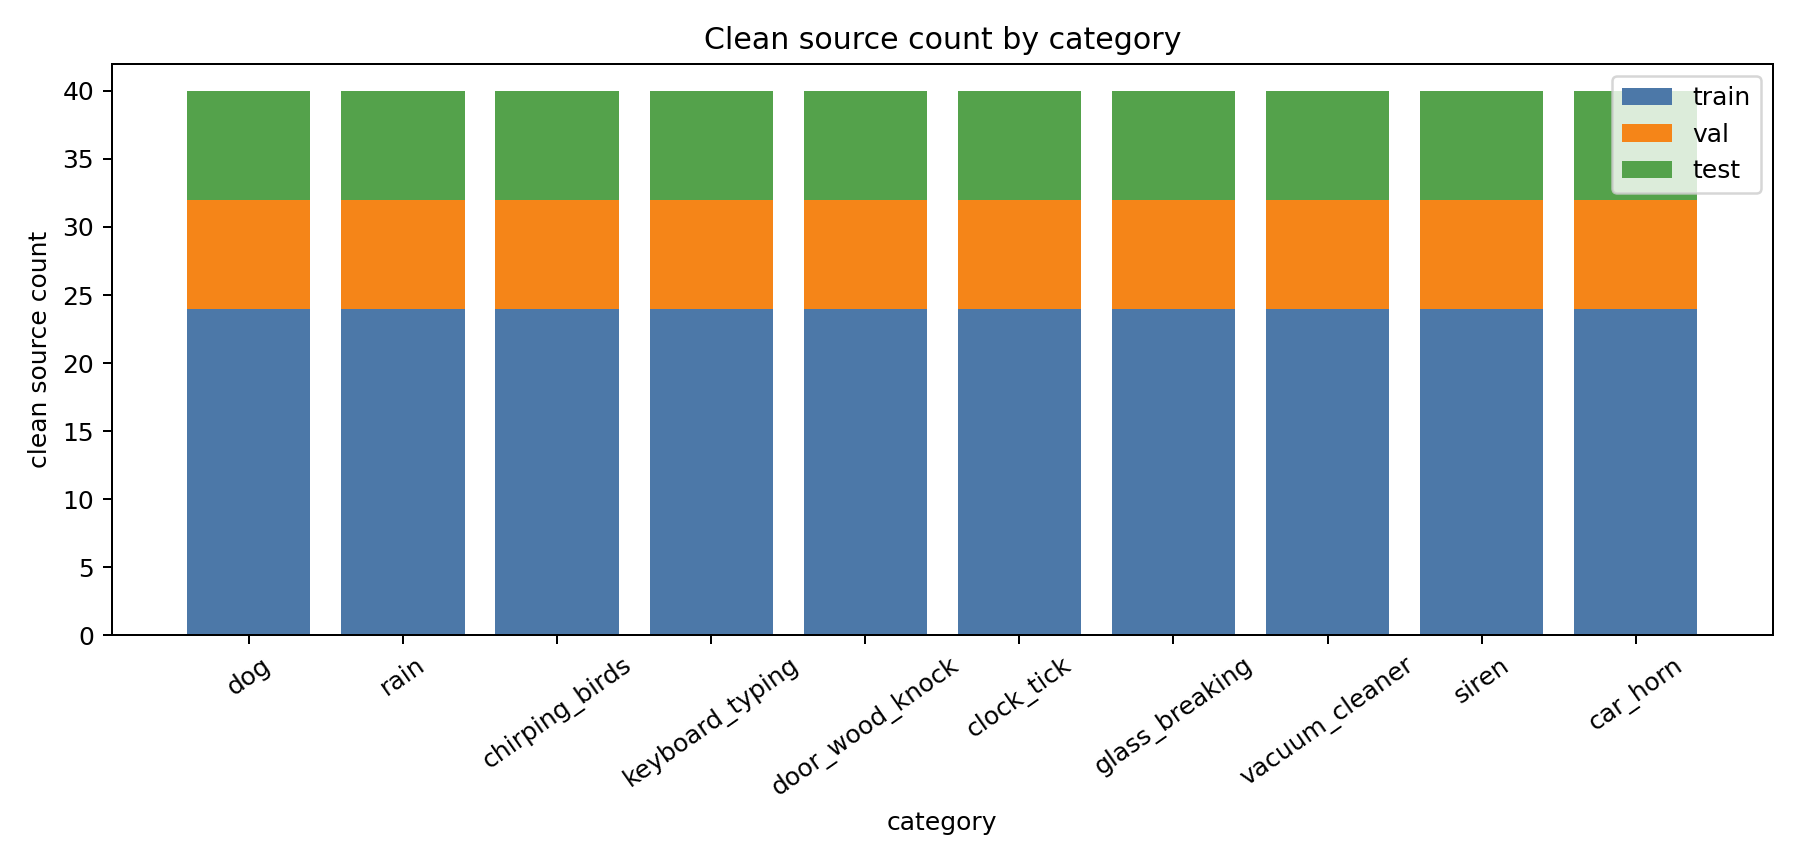
\includegraphics[width=\linewidth]{class_count.png}
    \caption{clean source类别数量}
  \end{subfigure}
  \hfill
  \begin{subfigure}[t]{0.48\textwidth}
    \centering
    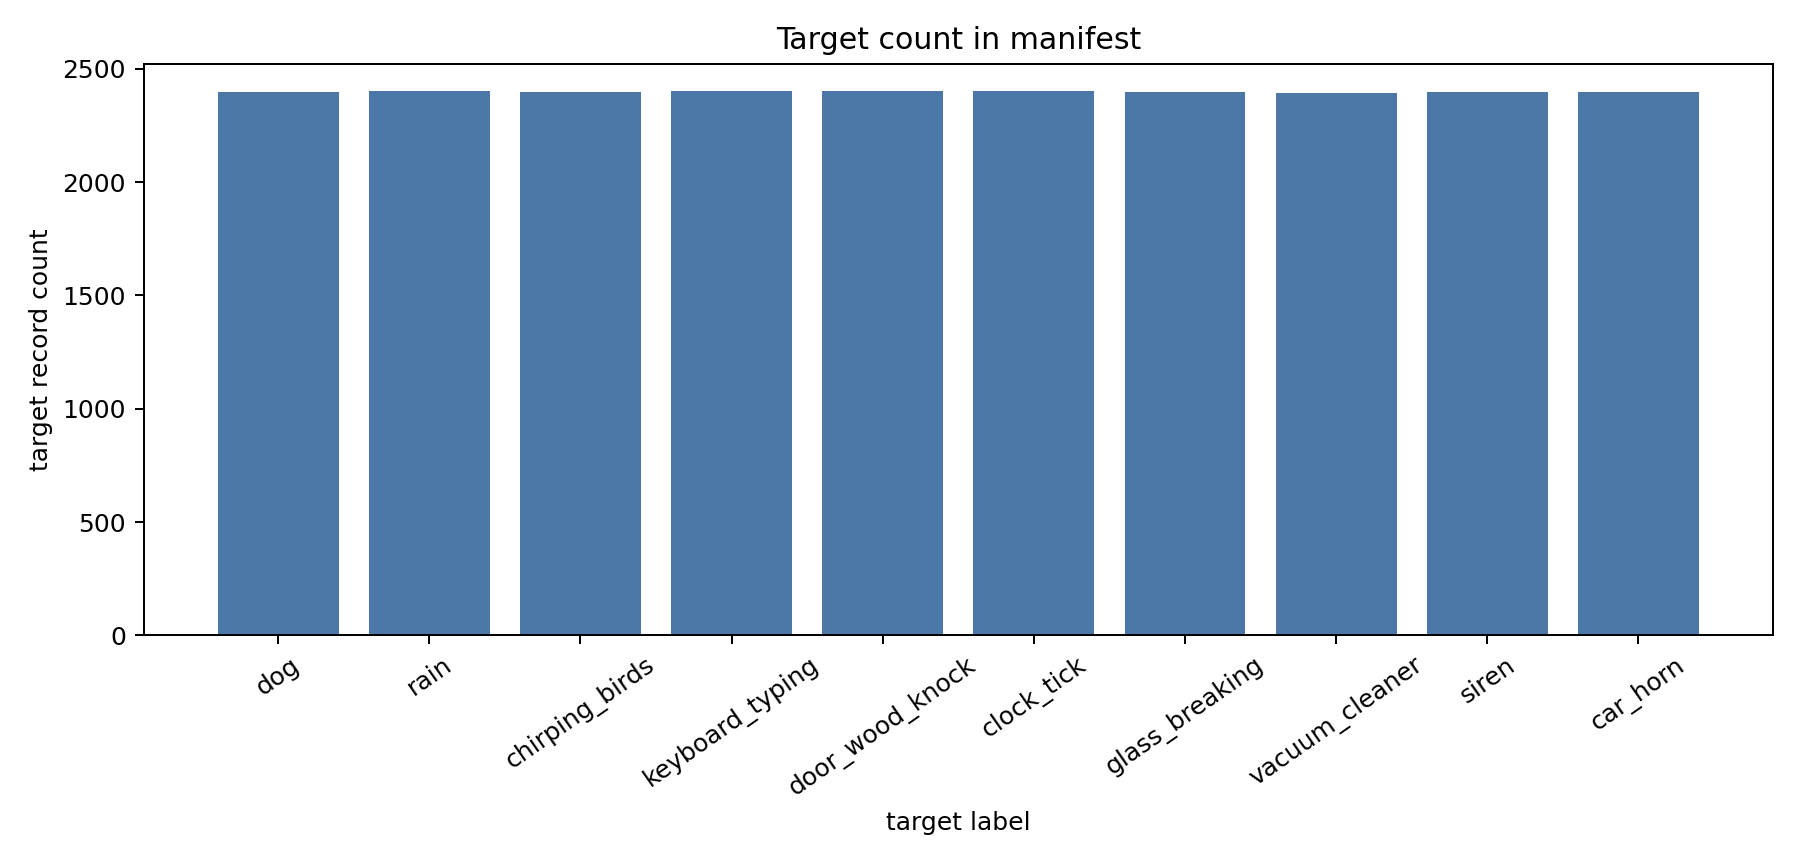
\includegraphics[width=\linewidth]{target_count.png}
    \caption{条件分离记录数量}
  \end{subfigure}
  \caption{所选类别与构造后target records的分布。}
  \label{fig:data-count}
\end{figure}

\subsection{预处理与二源混合}

原始音频先转换为16~kHz单声道，再裁剪或补零到80,000个采样点。clean source的RMS被归一化到0.1附近，同时检查峰值和低能量异常。两个源混合前，从$[-5,5]$~dB均匀采样相对增益$g$，然后按
\begin{equation}
  x_{\mathrm{mix}} = x_1 + 10^{g/20}x_2
\end{equation}
合成。合成结果再次进行峰值检查，避免写出音频时发生削波。

类别配对使用预先定义的compatibility list。每段mixture保存stem 0、stem 1及类别信息，并生成两条manifest记录：第一条以stem 0为target、stem 1为residual，第二条交换二者。这个设计让一段物理混合音频对应两个条件任务，也保证target和residual都有干净参考。

\begin{figure}[H]
  \centering
  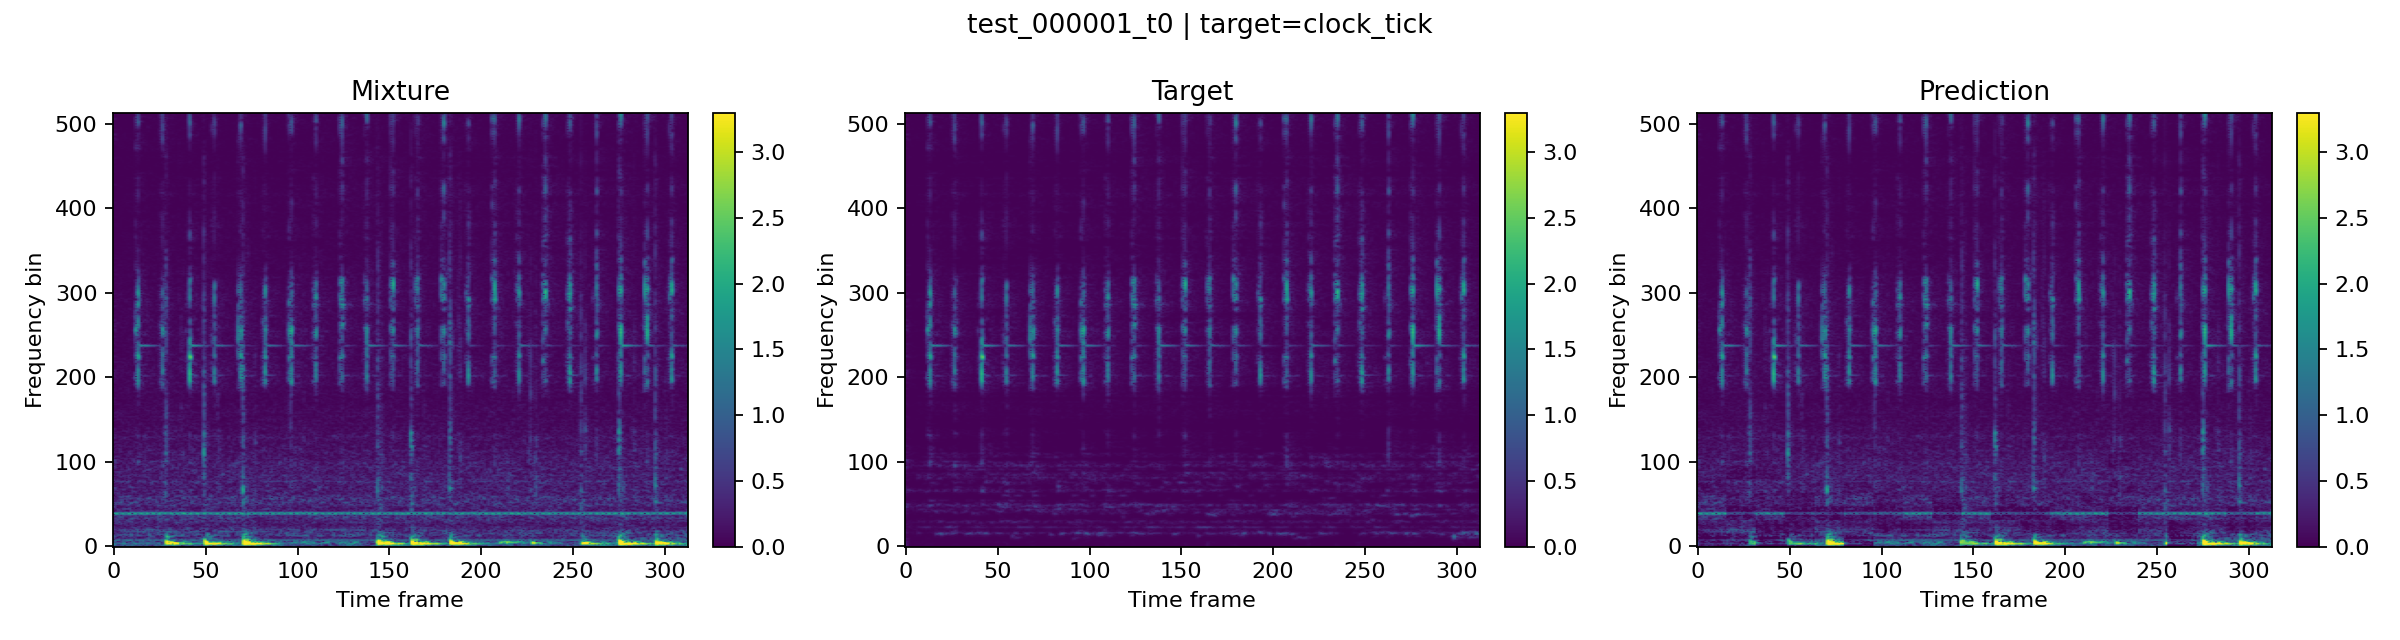
\includegraphics[width=0.94\textwidth]{dataset_triplet.png}
  \caption{一组2-mix样例的mixture、target和residual。相同mixture可通过label切换目标。}
  \label{fig:triplet}
\end{figure}

\subsection{划分与规模}

官方fold 1、2、3用于训练，fold 4用于验证，fold 5用于测试。划分在clean source层面完成，同一原始录音不会跨split出现。最终规模见表\ref{tab:data-scale}。训练集包含10,000条mixture和20,000条target records；验证集与测试集各包含1,000条mixture和2,000条target records。

\begin{table}[H]
  \centering
  \caption{ESC-50 2-mix数据规模。}
  \label{tab:data-scale}
  \begin{tabular}{lrrr}
    \toprule
    Split & Mixtures & Target records & Audio duration per record \\
    \midrule
    Train & 10,000 & 20,000 & 5 s \\
    Validation & 1,000 & 2,000 & 5 s \\
    Test & 1,000 & 2,000 & 5 s \\
    \bottomrule
  \end{tabular}
\end{table}

\subsection{数据质量核验}

合成数据的数量达到要求以后，我们又从“能否训练”和“是否可信”两个角度做了一轮核验。音频层面检查采样率、长度、有限数值、RMS与峰值；标注层面检查target label是否属于source labels、residual路径是否指向另一个stem；划分层面检查原始文件名和mixture id是否跨split重复。表\ref{tab:data-check}列出正式管线中的主要检查项。

\begin{table}[H]
  \centering
  \caption{2-mix数据质量检查。}
  \label{tab:data-check}
  \small
  \begin{tabularx}{0.95\textwidth}{p{3.0cm}X p{2.0cm}}
    \toprule
    检查项 & 判定方法 & 正式结果 \\
    \midrule
    采样率与长度 & 逐文件确认16~kHz、80,000 samples & 通过 \\
    静音与异常值 & 检查RMS、NaN、Inf及过低能量 & 通过 \\
    峰值与削波 & 统计绝对峰值并检查写盘后波形 & 通过 \\
    Mixture可加性 & 比较保存mixture与两个stem之和 & 通过 \\
    类别与路径 & 核对target、residual和source labels & 通过 \\
    Split泄漏 & 比较clean source文件名与fold归属 & 未发现交叉 \\
    类别均衡 & 统计每个split中的target label数量 & 基本均衡 \\
    \bottomrule
  \end{tabularx}
\end{table}

RMS归一化的目标是控制源间能量差，同时保留$[-5,5]$~dB相对增益带来的难度。过度归一化会让所有mixture变得相似，完全不控制能量又会产生大量近似单源样本。当前范围让较弱源仍有机会被听见，也覆盖了常见的主次声源关系。

官方fold在这里起到关键作用。ESC-50中的同类录音数量有限，如果先随机生成mixture再拆分，某条clean source可能同时进入训练和测试，模型会接触到测试声源的纹理。我们先按fold建立clean pool，再在各自pool内部配对，训练和测试之间保持源级隔离。后续所有实验都复用这套manifest，因此模型对照没有受到数据划分变化影响。

\section{方法}

\subsection{STFT幅度表示与音频重建}

对波形$x[n]$做短时傅里叶变换：
\begin{equation}
  X(\tau,k)=\sum_n x[n]w[n-\tau H]e^{-j2\pi kn/N},
\end{equation}
其中窗长和FFT点数$N=1024$，hop length $H=256$。5秒音频转换后得到$513\times313$的时频网格。复数频谱可写为
\begin{equation}
  X(\tau,k)=A(\tau,k)e^{j\phi(\tau,k)},
\end{equation}
其中$A=|X|$为幅度，$\phi=\arg X$为相位。模型输入使用经过缩放的对数幅度
\begin{equation}
  S=\sigma\log(1+A),
\end{equation}
以压缩不同能量区间。$\sigma$由训练集统计得到，数值为0.30338；训练与测试使用同一数值，特征最终截断到$[0,1]$。

模型输出$\hat S_{\mathrm{target}}$后，通过反变换得到预测幅度$\hat A_{\mathrm{target}}$，再与mixture phase组合：
\begin{equation}
  \hat X_{\mathrm{target}}=\hat A_{\mathrm{target}}e^{j\phi_{\mathrm{mix}}}.
\end{equation}
最后用iSTFT恢复波形。这里的相位来自mixture，模型没有学习target phase。幅度谱容易观察和训练，重建误差仍会受两源相位干涉影响。图\ref{fig:stft-pipeline}给出了完整处理链。

\begin{figure}[H]
  \centering
  \begin{tikzpicture}[node distance=6mm and 9mm]
    \node[spec] (wav) {波形\\$x[n]$};
    \node[mix,right=of wav] (stft) {STFT\\$X=A\,e^{j\phi}$};
    \node[spec,right=of stft] (logmag) {对数幅度\\$S=\sigma\log(1{+}A)$};
    \node[mix,right=of logmag] (model) {Mini-DiT\\$\hat S_{\mathrm{target}}$};
    \node[good,right=of model] (recon) {$\hat A\,e^{j\phi_{\mathrm{mix}}}$\\iSTFT};
    \node[good,right=of recon] (out) {目标波形\\$\hat x_{\mathrm{target}}$};
    \foreach \a/\b in {wav/stft,stft/logmag,logmag/model,model/recon,recon/out}
      \draw[flowarr] (\a) -- (\b);
    \node[spec,below=10mm of model,fill=blkloss] (phase) {mixture 相位\\$\phi_{\mathrm{mix}}$};
    \draw[condarr] (stft) |- (phase.west);
    \draw[condarr] (phase.east) -| (recon);
  \end{tikzpicture}
  \caption{从波形到对数幅度谱、经Mini-DiT预测目标幅度，再借用mixture相位重建波形。虚线表示相位来自mixture，模型只学习幅度。}
  \label{fig:stft-pipeline}
\end{figure}

\subsection{Conditional Flow Matching}

标准Flow Matching学习一个随时间变化的速度场。我们的路径起点$x_0$取mixture幅度谱，终点$x_1$取target幅度谱，在$t\in[0,1]$处线性插值得到
\begin{equation}
  x_t=(1-t)x_0+tx_1,
\end{equation}
对应的目标速度为
\begin{equation}
  v^*(x_t,t)=x_1-x_0.
\end{equation}
模型$v_\theta$同时接收$x_t$、mixture feature、时间$t$和target label $c$，速度损失为
\begin{equation}
  \mathcal L_{\mathrm{vel}}=\lVert v_\theta(x_t,t,x_{\mathrm{mix}},c)-v^*\rVert_1.
\end{equation}
训练中还加入endpoint loss，令$\hat x_1=x_t+(1-t)v_\theta$：
\begin{equation}
  \mathcal L_{\mathrm{end}}=\|\hat x_1-x_1\|_1.
\end{equation}
早期模型的总损失为$\mathcal L_{\mathrm{flow}}=\mathcal L_{\mathrm{vel}}+\mathcal L_{\mathrm{end}}$，速度项与endpoint项等权（各1.0）。后文提到的“Flow损失”均指这一组合项。推理从$x_0=x_{\mathrm{mix}}$出发，默认采用一次Euler更新。图\ref{fig:flow-path}把这条路径画成了mixture到target的连续移动。

\begin{figure}[H]
  \centering
  \begin{tikzpicture}[x=1.7cm,y=1.1cm]
    % 端点
    \node[spec,circle,minimum size=9mm] (x0) at (0,0) {$x_0$};
    \node[good,circle,minimum size=9mm] (x1) at (4,0) {$x_1$};
    \node[below=1mm of x0,font=\footnotesize,align=center] {mixture\\幅度谱};
    \node[below=1mm of x1,font=\footnotesize,align=center] {target\\幅度谱};
    % 路径
    \draw[flowarr,line width=0.8pt] (x0) -- (x1);
    % 中间点 x_t
    \fill[edgenavy] (2,0) circle (1.6pt);
    \node[font=\footnotesize,edgenavy] at (2,0.35) {$x_t=(1{-}t)x_0+t\,x_1$};
    % 速度场箭头
    \foreach \xx in {0.6,1.4,2.6,3.4}
      \draw[condarr,shorten >=0pt] (\xx,0.0) -- ++(0.5,0);
    \node[font=\footnotesize,edgenavy] at (2,-0.7) {$v^*=x_1-x_0$};
    % 推理标注
    \node[font=\footnotesize,align=center] at (2,0.95) {推理：从 $x_0$ 出发，1-step Euler 直达端点估计};
  \end{tikzpicture}
  \caption{Conditional Flow Matching的线性路径。训练随机采样$t$回归速度场$v^*$，推理从mixture端$x_0$出发。}
  \label{fig:flow-path}
\end{figure}

\subsection{Mini-DiT与类别条件}

输入频谱先按$16\times16$切成patch，映射到192维token序列。模型包含4个DiT block，每个block由序列mixer、MLP、LayerNorm和条件调制组成。时间$t$经过正弦位置编码和MLP，target label通过embedding转换成条件向量，两者相加后进入adaLN modulation。该模块产生shift、scale和gate，用于调节mixer与MLP两个残差分支。输出token恢复为空间网格，再投影成单通道速度场。图\ref{fig:arch}给出整体结构，并把单个block内的两种序列mixer并列展开。

self-attention baseline使用6头注意力，参数量为3,102,529。这个规模可以在单张GPU上完成训练，也为后续算子对照留下了相对稳定的预算。类别条件承担选择目标的作用；缺少label时，同一mixture中的两个源没有明确输出次序，监督目标会发生歧义。

\subsection{Mamba-style selective SSM}

状态空间模型通过隐藏状态$h_t$积累序列信息。离散形式可写成
\begin{align}
  h_t &= \bar A_t h_{t-1}+\bar B_t x_t,\\
  y_t &= C_t h_t + D x_t.
\end{align}
本项目的Mamba-style mixer先将token投影为内容分支$x$和门控分支$z$，在$x$上执行depthwise 1D convolution，再从当前输入生成步长$\Delta_t$以及$B_t,C_t$。状态沿token顺序递推，输出与$\mathrm{SiLU}(z)$相乘后投影回192维。$\Delta_t,B_t,C_t$随输入变化，使模型可以调节不同token对状态的写入和读取。

Mamba模型沿用4层、192维、相同patch和MLP配置，参数量为3,014,977。这里的Mamba-style mixer是纯PyTorch实现的selective SSM，未使用官方融合kernel，参数量按该实现统计。两种主干相差约2.8\%，仍属于同一轻量级区间。正式对照固定ESC-50 2-mix、STFT配置、Flow Matching目标、测试split和1-step推理，并补跑batch size一致的self-attention recheck。这样的设计能够回答当前预算下的算子差异，模型深度扩大后的结论仍需新的实验支持。

\begin{figure}[H]
  \centering
  \begin{tikzpicture}[node distance=5mm and 7mm]
    % ---- 上排：整体数据流 ----
    \node[spec] (xt) {$x_t$\\$513{\times}313$};
    \node[mlp,below=8mm of xt] (cond) {$t,\ c$\\嵌入};
    \node[spec,right=of xt] (patch) {Patchify\\$16{\times}16$};
    \node[mix,right=of patch] (blk) {DiT block\\$\times 4$};
    \node[spec,right=of blk] (unpatch) {反patch\\+ 投影};
    \node[good,right=of unpatch] (vout) {速度场\\$v_\theta$};
    \foreach \a/\b in {xt/patch,patch/blk,blk/unpatch,unpatch/vout}
      \draw[flowarr] (\a) -- (\b);
    \node[above=0.5mm of patch,font=\scriptsize] {$192$-d token};
    \draw[condarr] (cond.east) -| ($(blk.south)+(0,0)$);
    \node[font=\scriptsize,edgenavy] at ($(cond.east)!0.5!(blk.south)+(0.3,-0.35)$) {adaLN};
    % 分组框
    \begin{scope}[on background layer]
      \node[grp,fit=(xt)(patch)(blk)(unpatch)(vout)(cond),label={[font=\footnotesize]above:整体流程}] {};
    \end{scope}

    % ---- 下排：单个 DiT block 展开，两种 mixer 对照 ----
    \node[mix,below=16mm of blk,minimum width=22mm] (mixer) {序列 mixer};
    \node[mlp,right=of mixer,minimum width=16mm] (mlp) {MLP};
    \node[spec,left=of mixer,minimum width=12mm] (ln) {LayerNorm\\+ 调制};
    \draw[flowarr] (ln) -- (mixer);
    \draw[flowarr] (mixer) -- (mlp);
    \draw[condarr] (cond.south) |- (ln.west);
    \draw[flowarr,dotted] (blk.south) -- (mixer.north);

    % (a) self-attention
    \node[blk,fill=blkmix,below=12mm of ln,minimum width=30mm,align=left,font=\scriptsize]
      (sa) {(a) self-attention\\6 头，全局 token 交互};
    % (b) mamba
    \node[blk,fill=blkmix,below=12mm of mlp,minimum width=42mm,align=left,font=\scriptsize]
      (mb) {(b) Mamba-style SSM\\in\_proj\ $\to$\ depthwise conv\\$\to$\ 选择性状态 $\Delta_t,B_t,C_t$\ $\to$\ SiLU 门控};
    \draw[flowarr,dotted] (mixer.south) -- (sa.north);
    \draw[flowarr,dotted] (mixer.south) -- (mb.north);
  \end{tikzpicture}
  \caption{Mini-DiT整体结构与两种序列mixer。上排为$x_t$经patchify、4个DiT block到速度场$v_\theta$的数据流，$t$与label\,$c$经adaLN注入每个block；下排展开单个block，并对照(a)\,self-attention与(b)\,Mamba-style selective SSM两种mixer内部。虚线为条件流。}
  \label{fig:arch}
\end{figure}

\subsection{Waveform L1 continued training}

baseline阶段的Spec L1下降明显，SI-SDR没有同步改善。我们随后把预测endpoint转回波形，直接计算
\begin{equation}
  \mathcal L_{\mathrm{wav}}=\|\hat x_{\mathrm{target}}-x_{\mathrm{target}}\|_1.
\end{equation}
训练从Mamba best checkpoint继续，所有参数均参与更新，学习率降到$5\times10^{-5}$，训练10个epoch：
\begin{equation}
  \mathcal L_{\mathrm{W5}}=\mathcal L_{\mathrm{flow}}+0.1\mathcal L_{\mathrm{wav}}.
\end{equation}
波形重建仍使用mixture phase，因此该损失把频谱幅度误差经过iSTFT传播回模型。它能感知不同频率格子共同形成的时域误差，也会受到相位近似的影响。

\subsection{TF-mask与IRM辅助监督}

模型直接预测的target幅度在部分时频格子上超过mixture幅度。TF-mask clipping先计算
\begin{equation}
  M_{\mathrm{raw}}(t,f)=\frac{\hat A_{\mathrm{target}}(t,f)}{A_{\mathrm{mix}}(t,f)+\epsilon},
\end{equation}
再截断到$[0,1]$：
\begin{equation}
  M_{\mathrm{clip}}=\min(1,\max(0,M_{\mathrm{raw}})),\qquad
  \tilde A_{\mathrm{target}}=M_{\mathrm{clip}}A_{\mathrm{mix}}.
\end{equation}
这一步只修正幅度，phase继续取自mixture。由于复数频谱相加可能发生相位抵消，单源幅度并不总小于mixture幅度，因此clipping是一种有界工程先验，不是严格的物理约束。Wiener-style mask使用预测target和$residual\ proxy=\max(A_{\mathrm{mix}}-\hat A_{\mathrm{target}},0)$计算软比例。在这一proxy定义下，$p=1$与clipping在代数上等价；$p=2$会更强地压低低置信度格子。

训练数据中两个stem均已知。本项目采用功率比例形式的Oracle IRM：
\begin{equation}
  M_{\mathrm{IRM}}=\frac{A_{\mathrm{target}}^2}
  {A_{\mathrm{target}}^2+A_{\mathrm{residual}}^2+\epsilon}.
\end{equation}
Oracle IRM只用于诊断，不能由普通测试输入直接获得。正式微调令模型隐含的软mask接近$M_{\mathrm{IRM}}$：
\begin{equation}
  \mathcal L_{\mathrm{IRM}}=\left\lVert
  \mathrm{clip}\left(\frac{\hat A_{\mathrm{target}}}{A_{\mathrm{mix}}+\epsilon},0,1\right)
  -M_{\mathrm{IRM}}\right\rVert_1,
\end{equation}
最终损失为
\begin{equation}
  \mathcal L_{\mathrm{final}}=\mathcal L_{\mathrm{flow}}
  +0.1\mathcal L_{\mathrm{wav}}+0.1\mathcal L_{\mathrm{IRM}}.
\end{equation}
该阶段从waveform L1模型继续训练5个epoch，学习率为$3\times10^{-5}$，验证集最优权重出现在第2个epoch。图\ref{fig:mask-intuition}概括了预测幅度、mask约束和mixture幅度之间的关系。

\begin{figure}[H]
  \centering
  \begin{tikzpicture}[node distance=6mm and 12mm]
    \node[spec,align=center] (pred) {直接预测幅度\\$\hat A_{\mathrm{target}}$};
    \node[mix,right=of pred,align=center] (clip) {TF-mask 截断\\$M=\mathrm{clip}(\hat A/A_{\mathrm{mix}},0,1)$\\$\tilde A=M\,A_{\mathrm{mix}}$};
    \node[loss,right=of clip,align=center] (irm) {IRM 辅助监督\\$M_{\mathrm{IRM}}=\dfrac{A_t^2}{A_t^2+A_r^2+\epsilon}$};
    \draw[flowarr] (pred) -- (clip);
    \draw[flowarr] (clip) -- (irm);
    \node[below=8mm of clip,font=\footnotesize,align=center,text width=0.8\textwidth]
      {截断把预测幅度约束在mixture幅度以内；IRM用训练时已知的两个stem给出理想比例，作为辅助损失$\mathcal L_{\mathrm{final}}=\mathcal L_{\mathrm{flow}}+0.1\mathcal L_{\mathrm{wav}}+0.1\mathcal L_{\mathrm{IRM}}$。};
  \end{tikzpicture}
  \caption{TF-mask与IRM辅助监督的关系。Oracle IRM使用真实stem，作为诊断参考和训练监督。}
  \label{fig:mask-intuition}
\end{figure}

\subsection{Target与residual输出}

模型显式输出prediction target。residual通过二源可加性得到：
\begin{equation}
  \hat x_{\mathrm{residual}}=x_{\mathrm{mix}}-\hat x_{\mathrm{target}}.
\end{equation}
这个处理保证两路输出相加后与mixture对齐，也让系统形成可试听的二源结果。它没有单独学习residual目标，target中的误差会以相反符号进入residual。Week6的结果表明，target指标上升时residual指标可能下降，这一点将在第\ref{sec:results}节展开。

\section{实验设置与评价方法}

\subsection{训练配置}

所有主实验使用同一数据划分和频谱配置。self-attention与Mamba从随机初始化训练，Mamba实验采用batch size 48，并补跑相同batch的self-attention recheck。waveform L1和IRM阶段从前一阶段best checkpoint继续训练。表\ref{tab:training-setting}列出关键设置。

\begin{table}[H]
  \centering
  \caption{主实验训练配置。}
  \label{tab:training-setting}
  \small
  \resizebox{0.98\textwidth}{!}{\begin{tabular}{lcccc}
    \toprule
    阶段 & 初始化 & Epochs & Learning rate & Loss \\
    \midrule
    Self-attention baseline & Random & 40 & $2\times10^{-4}$ & Flow \\
    Mamba-style SSM & Random & 40 & $2\times10^{-4}$ & Flow \\
    Waveform continued training & Mamba best & 10 & $5\times10^{-5}$ & Flow + 0.1 Wave \\
    IRM continued training & Waveform best & 5 & $3\times10^{-5}$ & Flow + 0.1 Wave + 0.1 IRM \\
    \bottomrule
  \end{tabular}}
\end{table}

优化器为AdamW，weight decay 0.01，梯度范数裁剪为1.0，GPU训练启用自动混合精度。验证阶段使用固定随机种子采样$t$，减小不同epoch之间的随机波动。checkpoint按验证损失选择，测试集只用于最终评价。

\subsection{评价指标}

Spec L1计算预测特征与target特征的平均绝对误差；两者均为缩放并截断到$[0,1]$的对数幅度谱。Wave L1在iSTFT重建后逐采样点计算误差。二者越低越好，数值受特征缩放和波形幅值影响，只适合同一数据协议下比较。

SI-SDR实现先分别去除估计信号与参考信号的均值，再将$\hat s$投影到$s$上\cite{leroux2019sisdr}：
\begin{align}
  s_{\mathrm{target}}&=\frac{\langle\hat s,s\rangle}{\|s\|^2}s,\\
  e_{\mathrm{noise}}&=\hat s-s_{\mathrm{target}},\\
  \mathrm{SI\text{-}SDR}&=10\log_{10}\frac{\|s_{\mathrm{target}}\|^2}{\|e_{\mathrm{noise}}\|^2}.
\end{align}
它消除整体缩放的影响，数值越高表示输出中的目标成分相对误差更强。测试集上直接使用mixture作为估计时，Target SI-SDR约为0.004~dB。最终模型达到2.535~dB，对应约2.531~dB的SI-SDR improvement。

MR-STFT指标使用$n_{\mathrm{fft}}=256,512,1024$三组窗口，在$\log(1+|\mathrm{STFT}|)$上计算L1后取平均。它用于观察不同时间--频率分辨率上的误差。试听和类别统计补充平均数难以呈现的个体差异。

\subsection{比较口径}

主结果均来自2,000条test target records、1-step inference。推理步数消融只使用512条test records，因而单独成表。Oracle IRM使用ground-truth target与residual，是当前IRM定义和mixture phase重建方式下的oracle参考，不构成所有幅度估计方法的严格上界。不同数据集、采样率、提示模态或指标实现得到的数值不适合直接横向比较。

\section{实验结果与分析}\label{sec:results}

\subsection{第一个baseline带来的判断}

self-attention baseline训练40个epoch后，Target Spec L1从mixture参考的0.05708降到0.03539，Target Wave L1从0.04200降到0.03203。两个L1指标分别有66.25\%和69.70\%的样例获得改善。Target SI-SDR为$-0.419$~dB，比mixture参考低0.424~dB，只有50.4\%样例在该指标上改善。

\begin{figure}[H]
  \centering
  \begin{subfigure}[t]{0.48\textwidth}
    \centering
    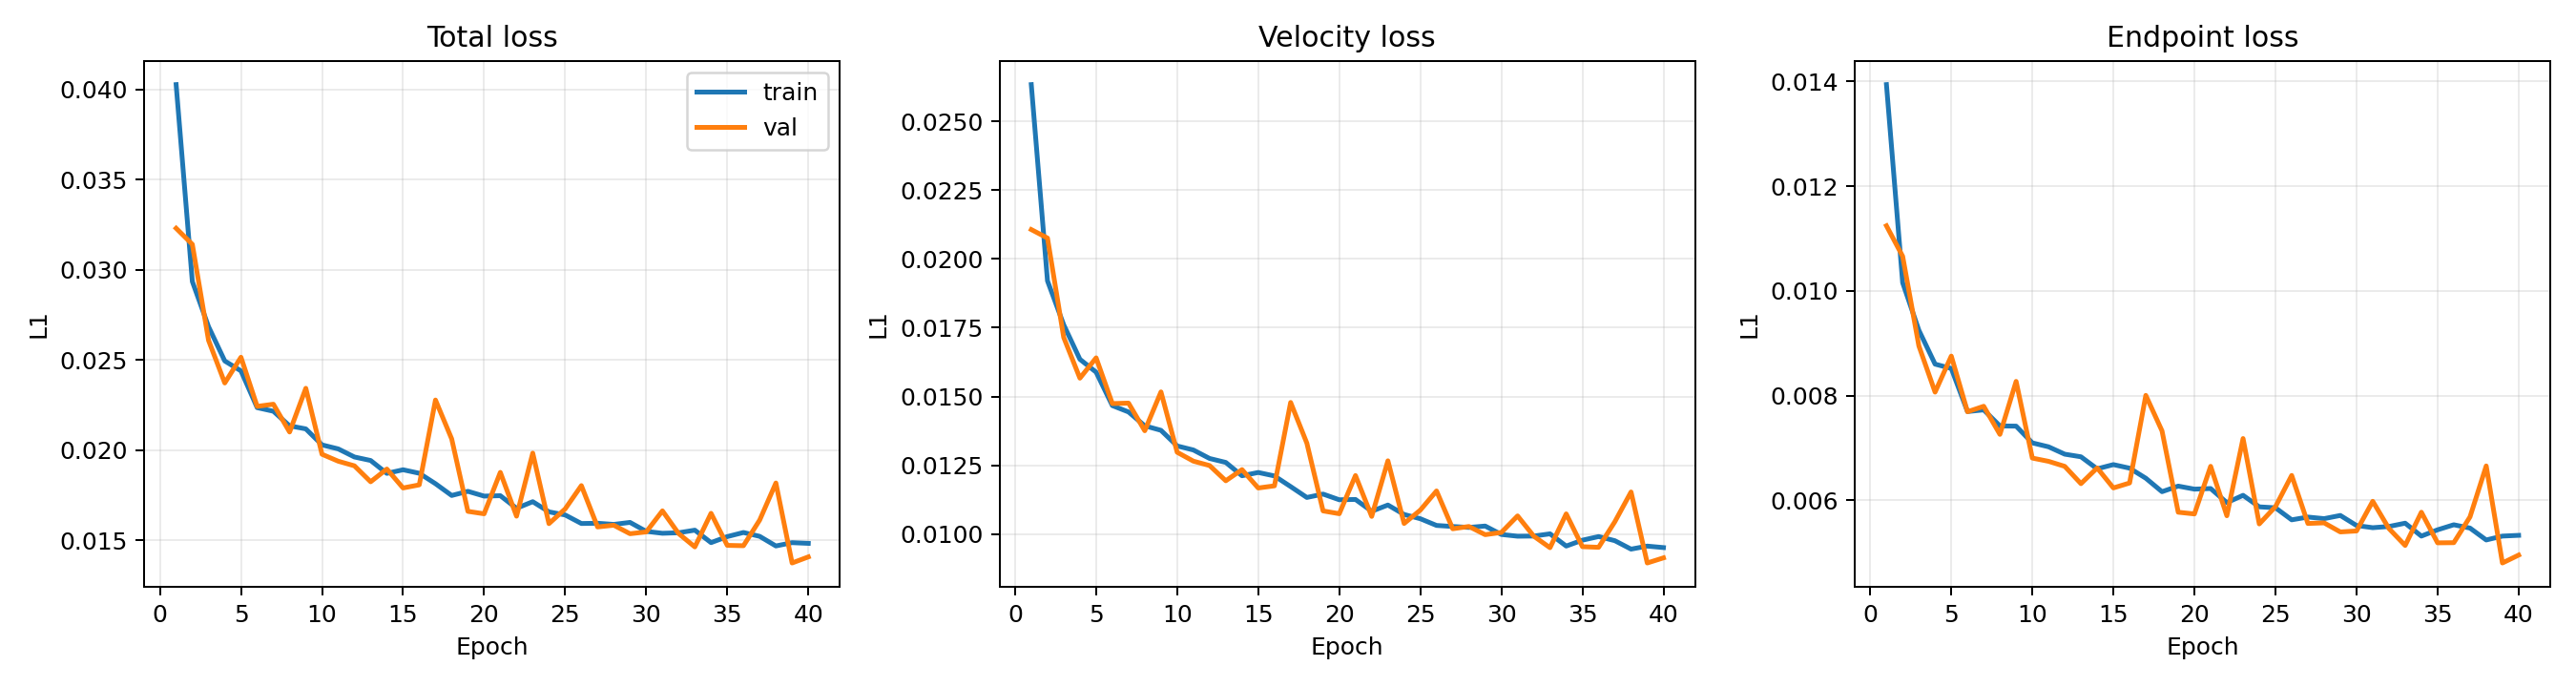
\includegraphics[width=\linewidth]{week3_training_curves.png}
    \caption{训练与验证损失}
  \end{subfigure}
  \hfill
  \begin{subfigure}[t]{0.48\textwidth}
    \centering
    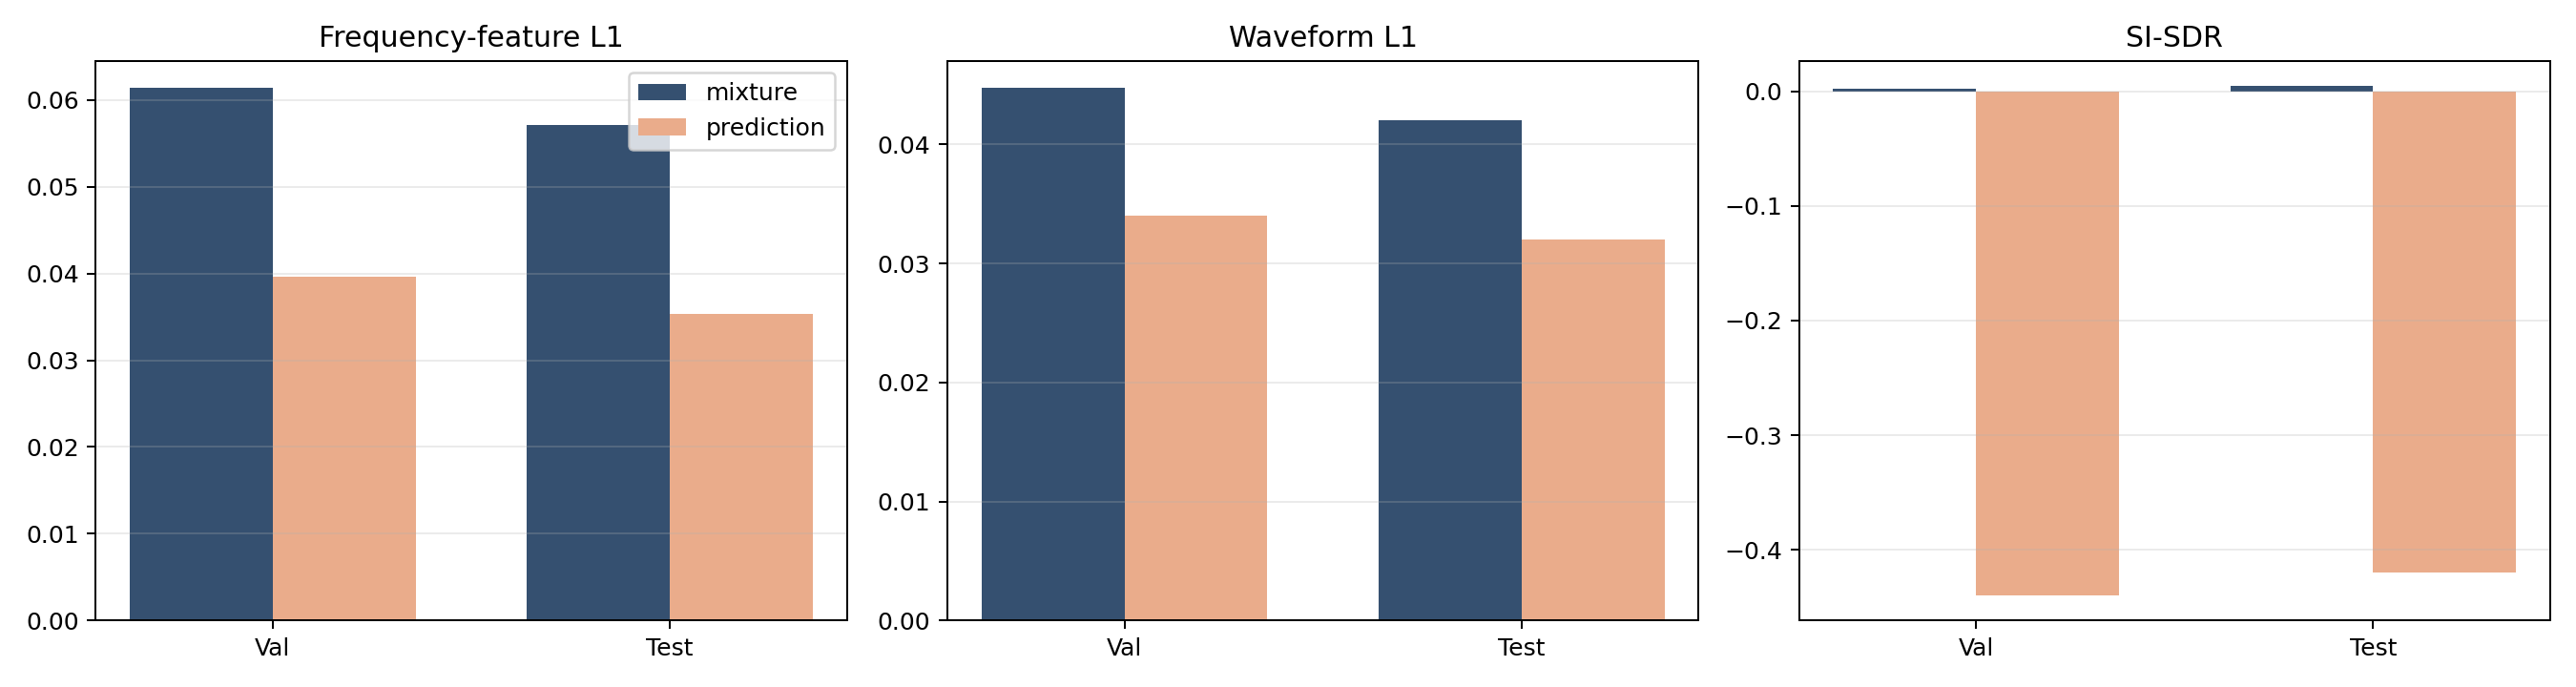
\includegraphics[width=\linewidth]{week3_eval_overview.png}
    \caption{完整测试集指标}
  \end{subfigure}
  \caption{Self-attention baseline的训练和测试表现。}
  \label{fig:week3-result}
\end{figure}

训练过程稳定，模型确实学到了target幅度的平均结构。SI-SDR的方向提醒我们，逐格L1可能通过平滑或削弱局部能量获得较低误差，声音的目标成分与干扰比例仍然较差。后续模型选择因此以SI-SDR和Wave L1为主，Spec L1继续保留，用于观察频谱层面的取舍。

\subsection{Self-attention与Mamba-style SSM}

Week4补跑的self-attention recheck与Mamba使用同一batch size和评估脚本。Mamba在三项target指标上都取得更好结果：Spec L1为0.03047，Wave L1为0.02815，SI-SDR为0.642~dB；self-attention recheck分别为0.03600、0.03378和$-1.418$~dB。

\begin{figure}[H]
  \centering
  \begin{subfigure}[t]{0.49\textwidth}
    \centering
    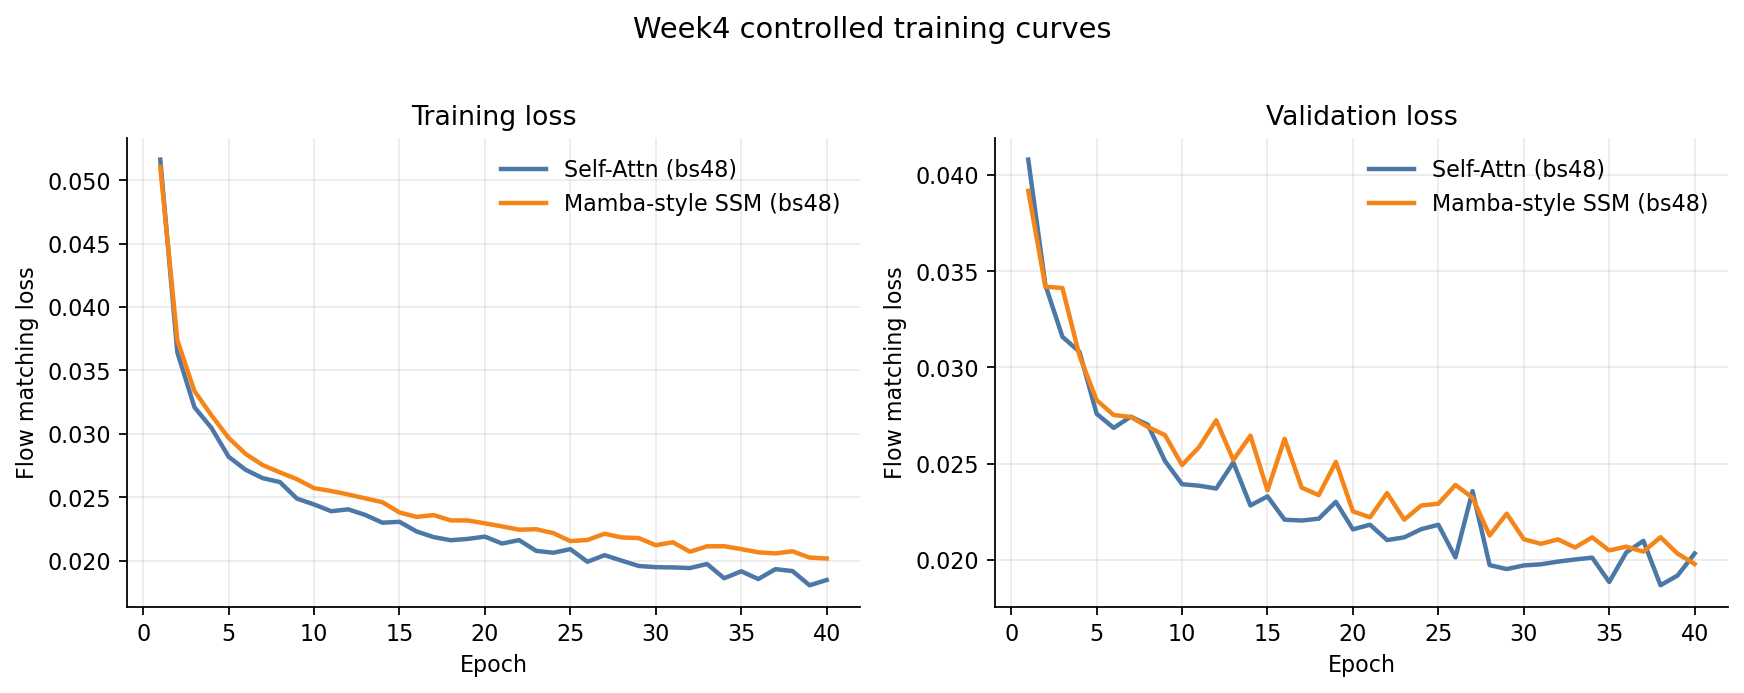
\includegraphics[width=\linewidth]{week4_training_curves.png}
    \caption{两种算子的训练曲线}
  \end{subfigure}
  \hfill
  \begin{subfigure}[t]{0.49\textwidth}
    \centering
    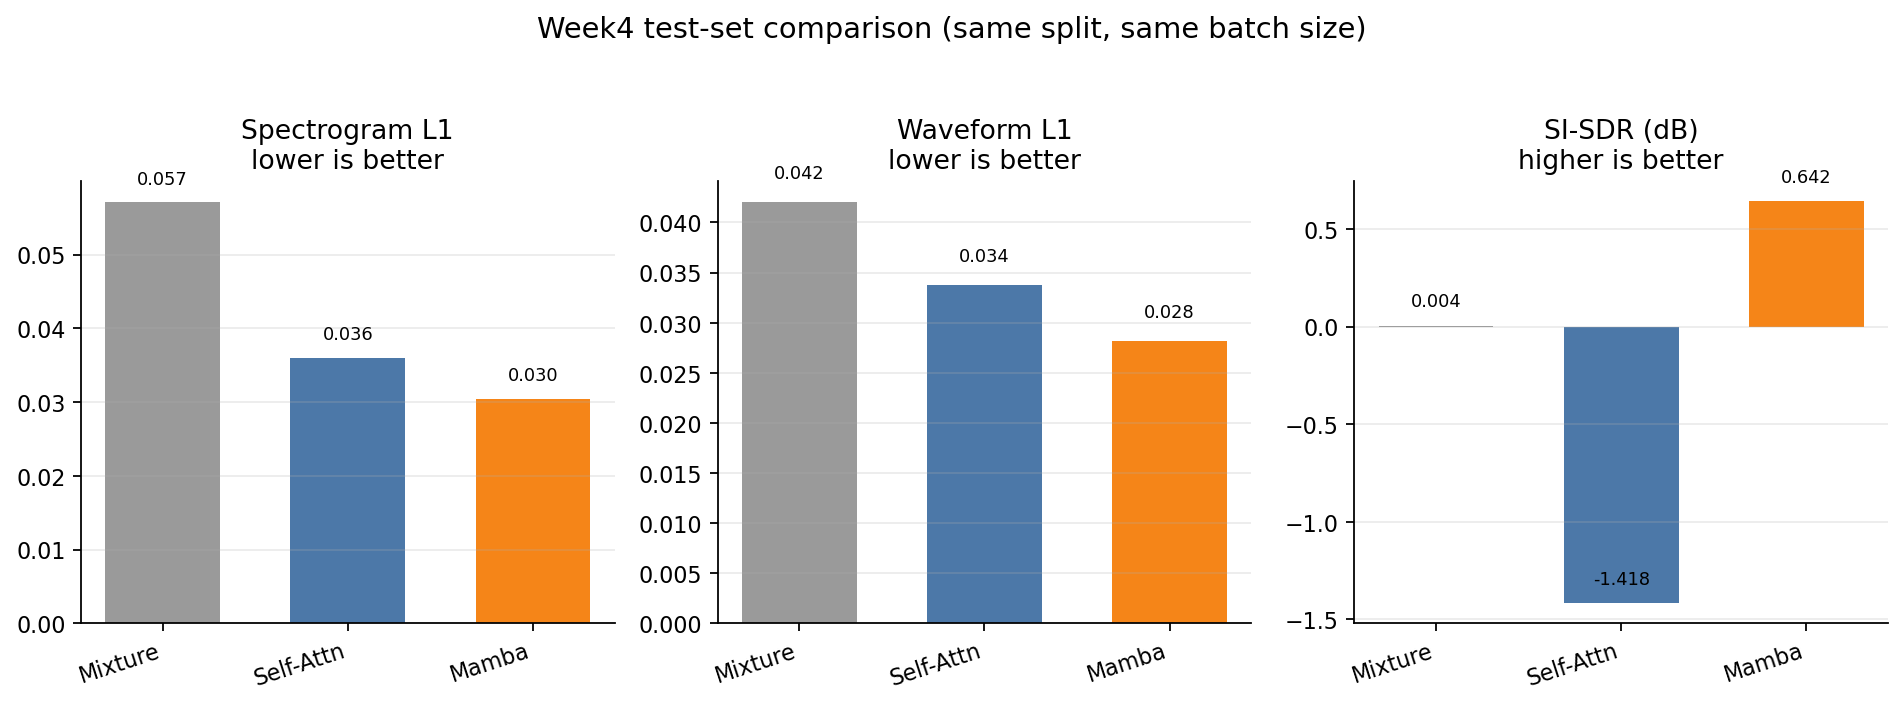
\includegraphics[width=\linewidth]{week4_metrics.png}
    \caption{测试指标对照}
  \end{subfigure}
  \caption{相近参数量下self-attention与Mamba-style SSM的比较。}
  \label{fig:week4-result}
\end{figure}

Mamba将Target SI-SDR首次提高到mixture参考以上，表明当前Mamba-style实现更适合这组训练设置。数据量约为20,000条target records，主干只有4层，频谱patch按固定顺序展开。实验没有单独分离递推结构、优化稳定性和参数分配的影响，因此无法把增益归因于某一个机制。扩大self-attention深度、数据规模或训练轮数后，两种算子的相对位置可能改变。

\subsection{模型规模与计算代价}

两种主干的参数量接近，运行代价差异却很大。同一服务器上的单次训练记录显示，self-attention recheck约为0.28小时，纯PyTorch selective SSM实现约为13.21小时。图\ref{fig:runtime}展示了这组记录。显式状态循环逐token执行，无法充分利用融合CUDA kernel，理论上的线性复杂度没有转化成当前代码的训练速度。这组时间用于说明当前实现，不作为通用性能基准。

\begin{figure}[H]
  \centering
  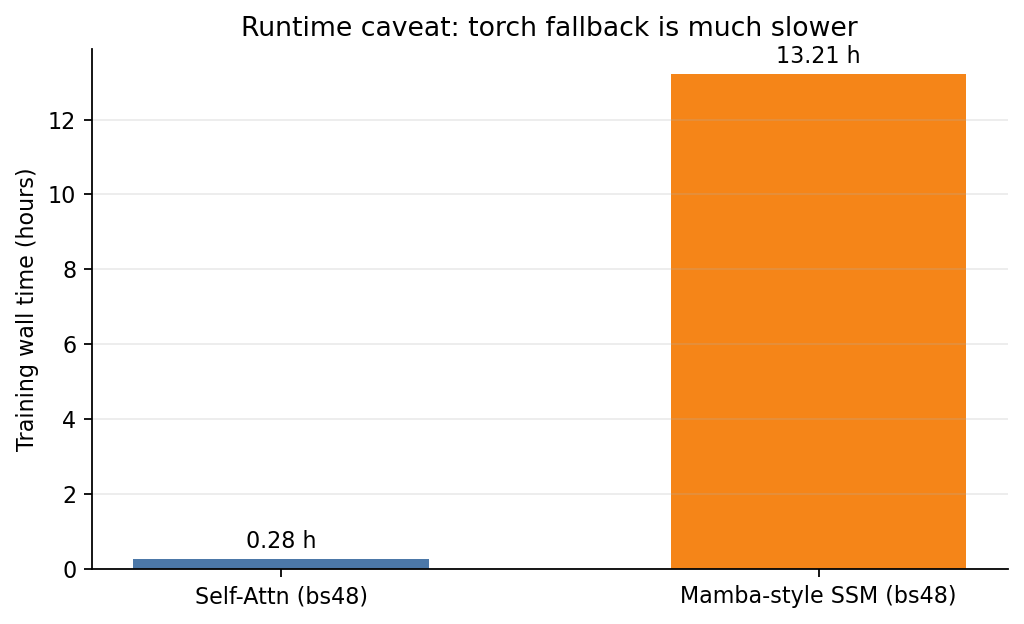
\includegraphics[width=0.72\textwidth]{runtime_comparison.png}
  \caption{正式训练记录中的运行时间。数值反映当前PyTorch实现。}
  \label{fig:runtime}
\end{figure}

这项观察使本项目的结论更具体。Mamba-style SSM带来了质量收益，当前实现付出了更高训练时间。参数量只能反映模型存储和一部分计算规模，kernel实现、内存访问和并行方式也会决定真实效率。若把Mamba作为部署方案，还需要在兼容硬件上使用融合scan kernel，并重新测量吞吐量、显存和实时率。

我们仍保留这次算子实验，因为它回答了课程项目最初提出的建模问题：在相近参数预算下，selective SSM能否改善频谱序列的分离质量。速度数据则帮助我们划清工程结论，当前版本适合做结构验证，尚未形成推理效率优势。

\subsection{Waveform L1带来的变化}

从Mamba best checkpoint继续训练后，Target Wave L1从0.02815降到0.02721，Target SI-SDR从0.642提高到1.417~dB，Residual SI-SDR达到1.975~dB。Target Spec L1从0.03047升到0.03097，MR-STFT距离也有小幅上升。

\begin{figure}[H]
  \centering
  \begin{subfigure}[t]{0.49\textwidth}
    \centering
    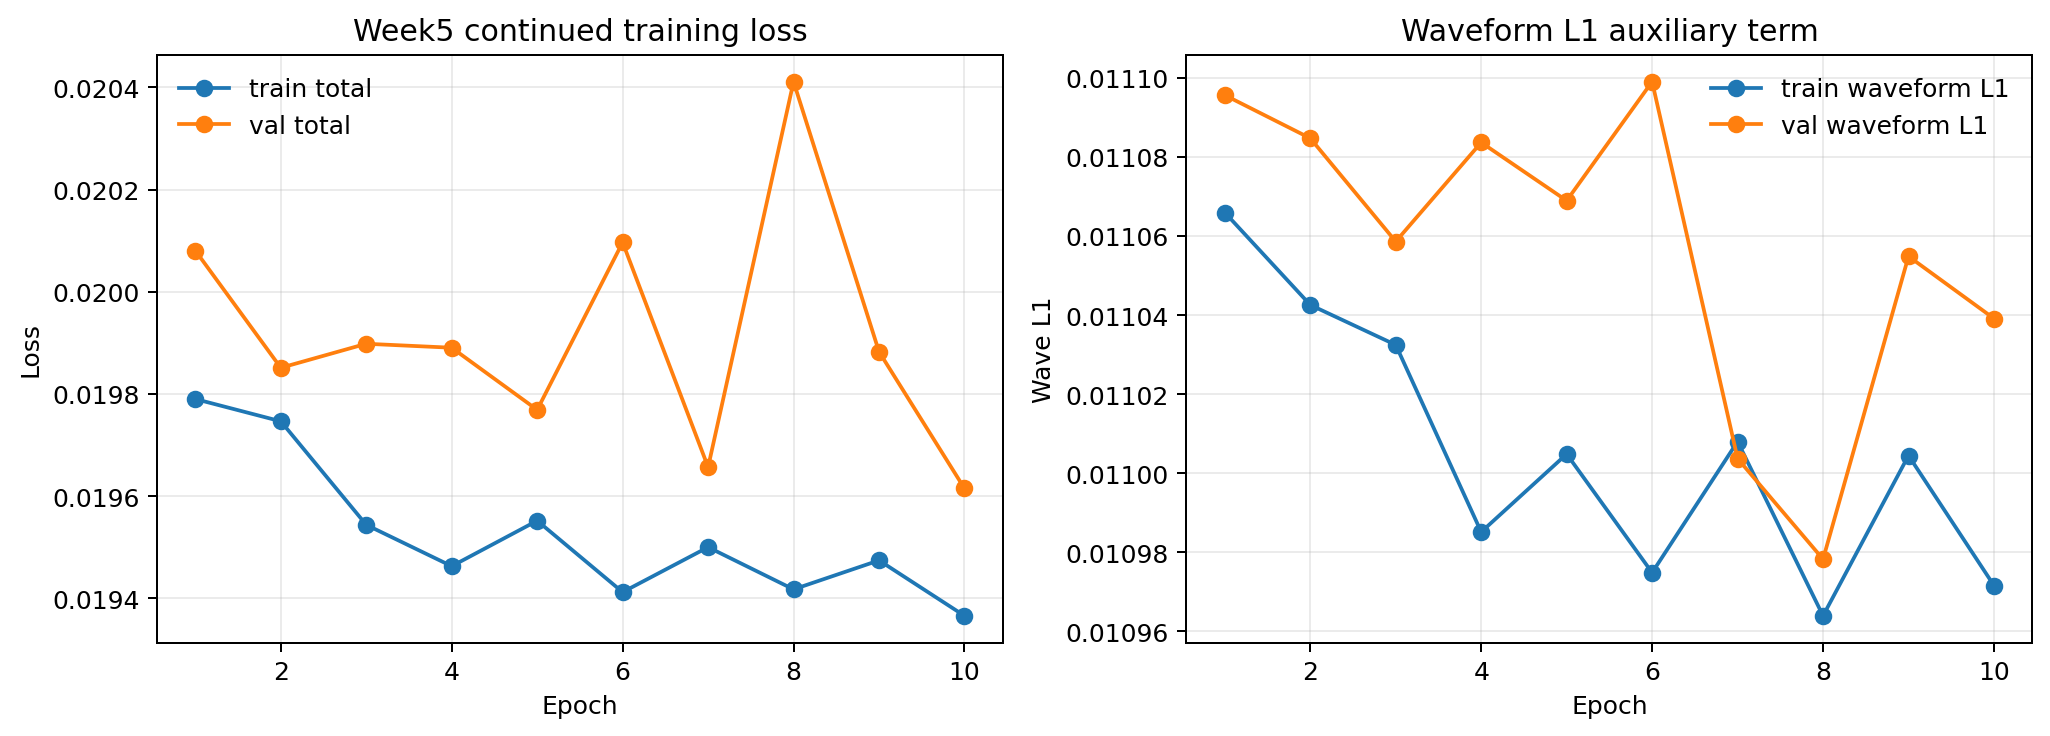
\includegraphics[width=\linewidth]{week5_training_curves.png}
    \caption{continued training曲线}
  \end{subfigure}
  \hfill
  \begin{subfigure}[t]{0.49\textwidth}
    \centering
    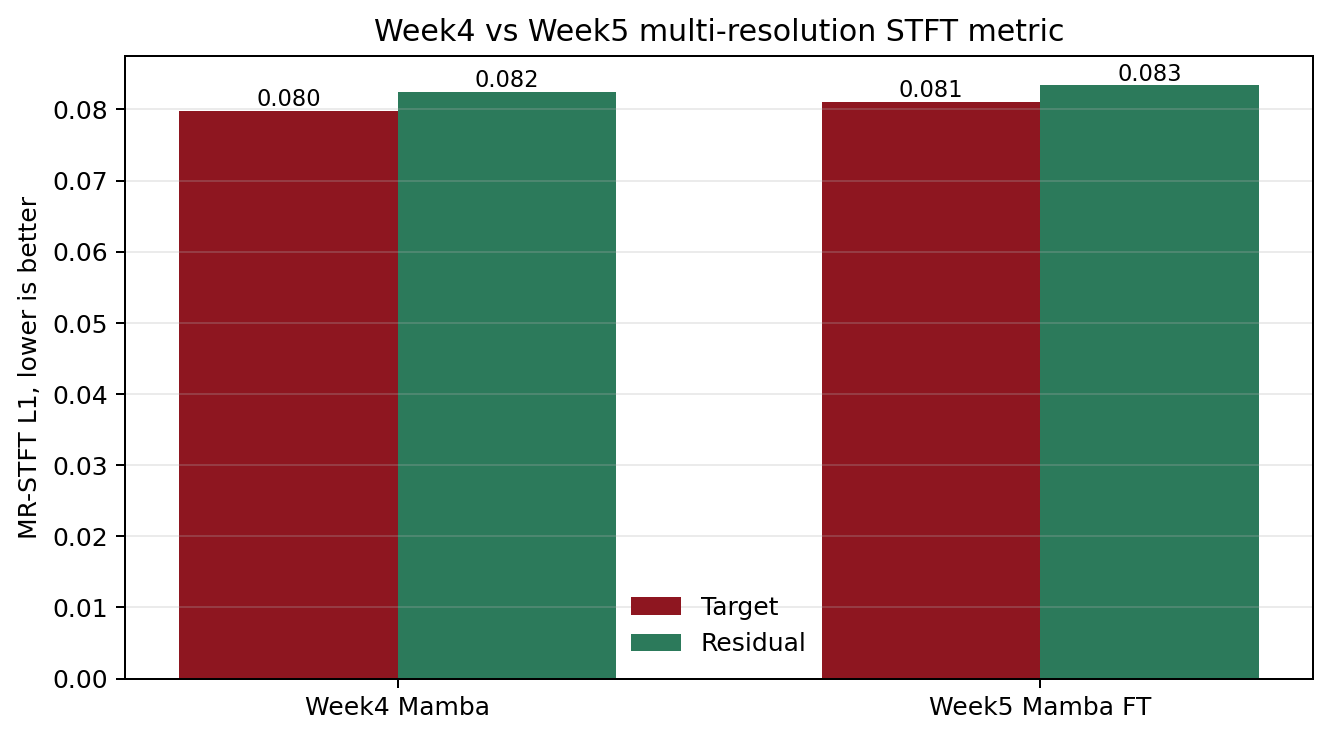
\includegraphics[width=\linewidth]{mrstft_comparison.png}
    \caption{离线MR-STFT比较}
  \end{subfigure}
  \caption{加入waveform L1后的训练与频谱指标变化。}
  \label{fig:week5-result}
\end{figure}

这组结果呈现了清楚的目标取舍。新增波形损失让优化更关注iSTFT后的采样点误差，Wave L1和SI-SDR获得收益；单尺度Spec L1和多尺度MR-STFT没有同步下降。音频质量无法由一个频谱L1完整概括，训练目标需要和最终使用场景保持联系。

\subsection{推理步数消融}

我们在同一512条test records上比较1、2、4、8步Euler推理。步数增加后Spec L1从0.03076缓慢降到0.03040，Target SI-SDR则从1.413降到1.173~dB，Wave L1也没有稳定改善。结果见图\ref{fig:steps}和表\ref{tab:steps}。

\begin{figure}[H]
  \centering
  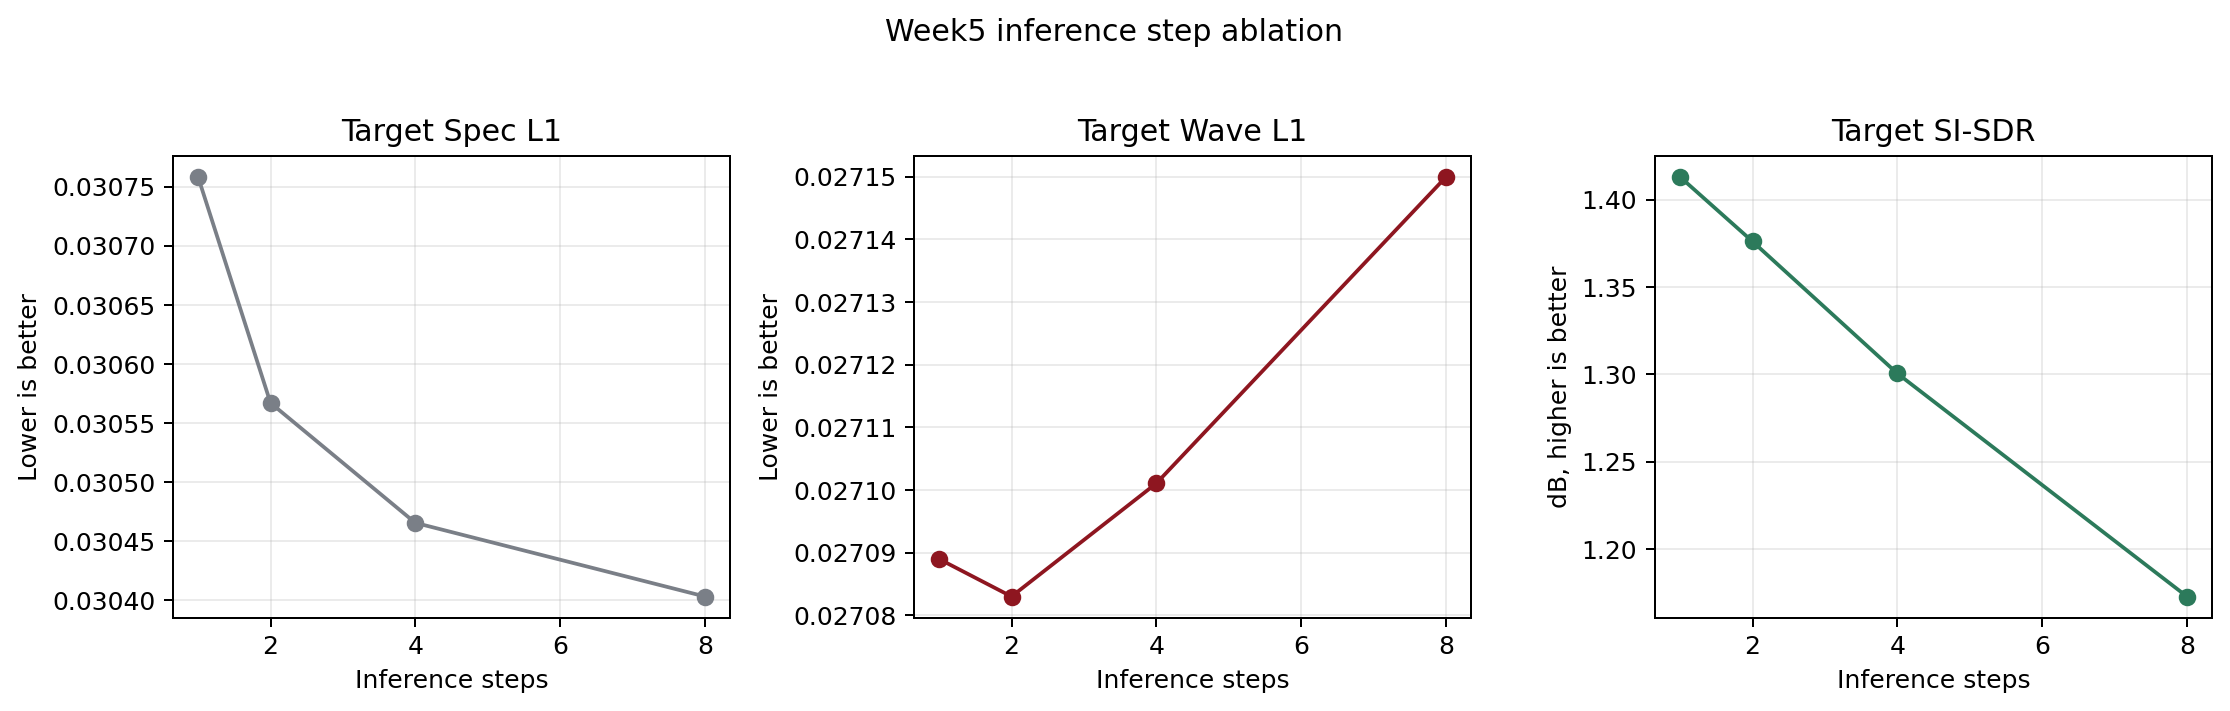
\includegraphics[width=0.9\textwidth]{inference_steps.png}
  \caption{1/2/4/8-step推理消融，使用512条test records。}
  \label{fig:steps}
\end{figure}

\begin{table}[H]
  \centering
  \caption{推理步数消融。}
  \label{tab:steps}
  \begin{tabular}{rrrrr}
    \toprule
    Steps & Target Spec L1 & Target Wave L1 & Target SI-SDR & Residual SI-SDR \\
    \midrule
    1 & 0.03076 & 0.02709 & 1.413 & 2.047 \\
    2 & 0.03057 & 0.02708 & 1.376 & 2.034 \\
    4 & 0.03047 & 0.02710 & 1.301 & 1.988 \\
    8 & 0.03040 & 0.02715 & 1.173 & 1.896 \\
    \bottomrule
  \end{tabular}
\end{table}

当前速度场在训练时回归直线路径，1-step对应直接endpoint估计。多步结果显示频谱平均误差略降，波形指标却逐步受损。一种可能的原因是逐步积分产生了训练时较少出现的中间状态。最终协议据此保留1-step。

\subsection{TF-mask后处理与Oracle诊断}

TF-mask clipping应用在waveform L1模型上时，Target SI-SDR从1.417提高到1.431~dB，增量约0.013~dB。Wiener $p=1$与clipping结果一致；Wiener $p=2$把Spec L1压到0.02982，Target SI-SDR降到0.422~dB。更强的功率掩码抑制了部分真实target能量，再次出现频谱L1和音频指标方向不同的情况。

Oracle IRM的Target SI-SDR为14.869~dB，Residual SI-SDR为14.362~dB。它使用真实stem计算mask，无法在普通测试输入中获得。该结果用于估计所选功率比例mask在mixture phase条件下的潜力。Oracle输出仍借用mixture phase，因此无法完美重建target。

\begin{figure}[H]
  \centering
  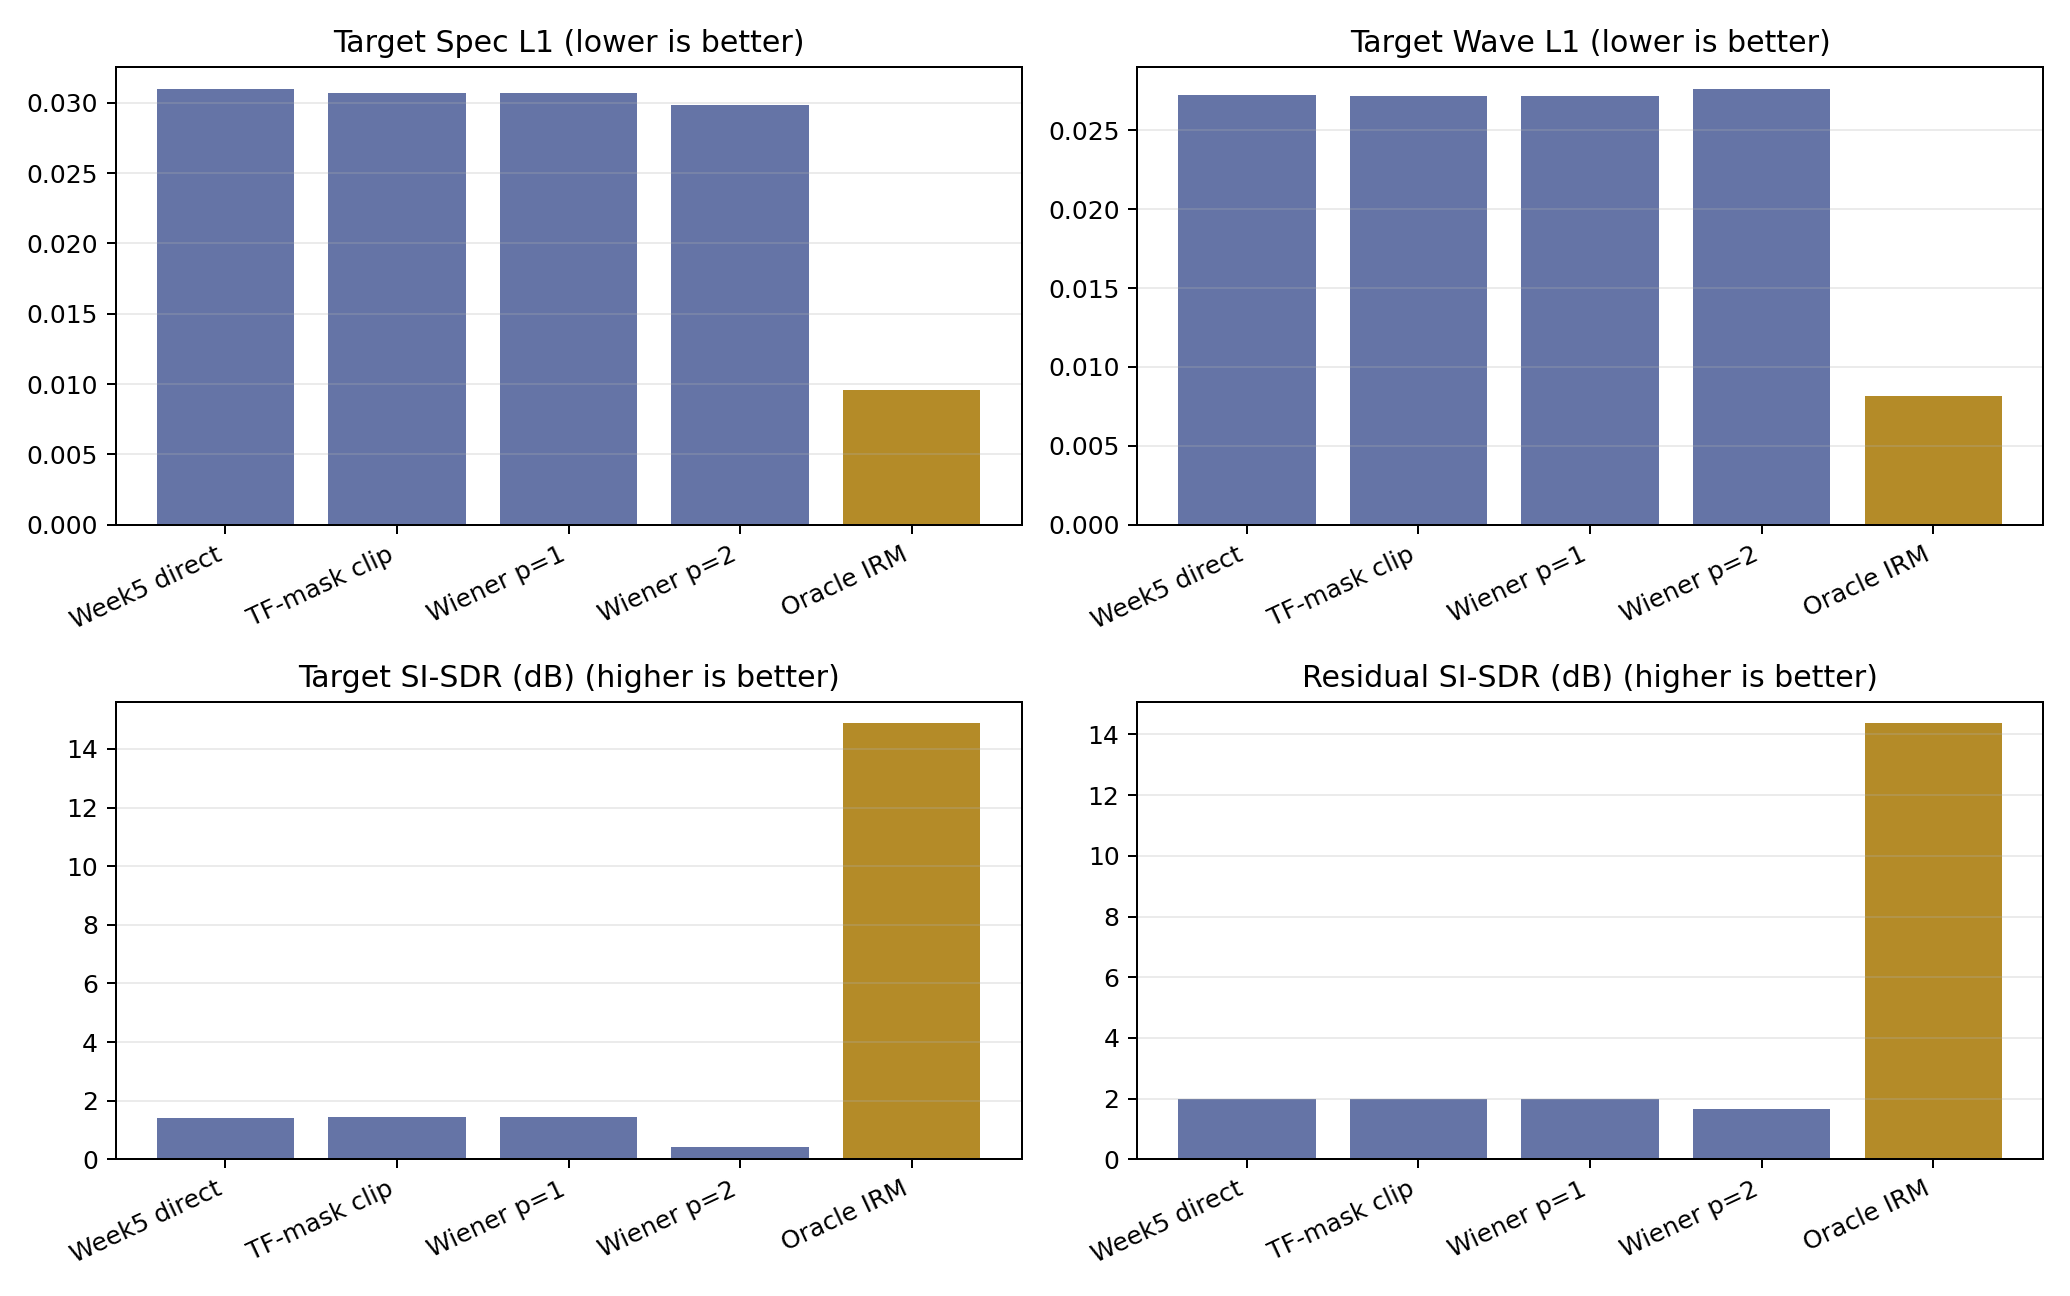
\includegraphics[width=0.88\textwidth]{tfmask_metrics.png}
  \caption{Waveform L1模型上的TF-mask、Wiener mask和Oracle IRM。}
  \label{fig:tfmask}
\end{figure}

\subsection{IRM辅助训练与最终结果}

Oracle诊断促使我们把mask监督放进训练。IRM continued training的direct输出达到2.528~dB Target SI-SDR，配合clipping后达到2.535~dB，Wave L1为0.02663，Spec L1为0.03064。后处理只贡献约0.007~dB，主要收益来自IRM辅助损失对模型参数的更新。

\begin{figure}[H]
  \centering
  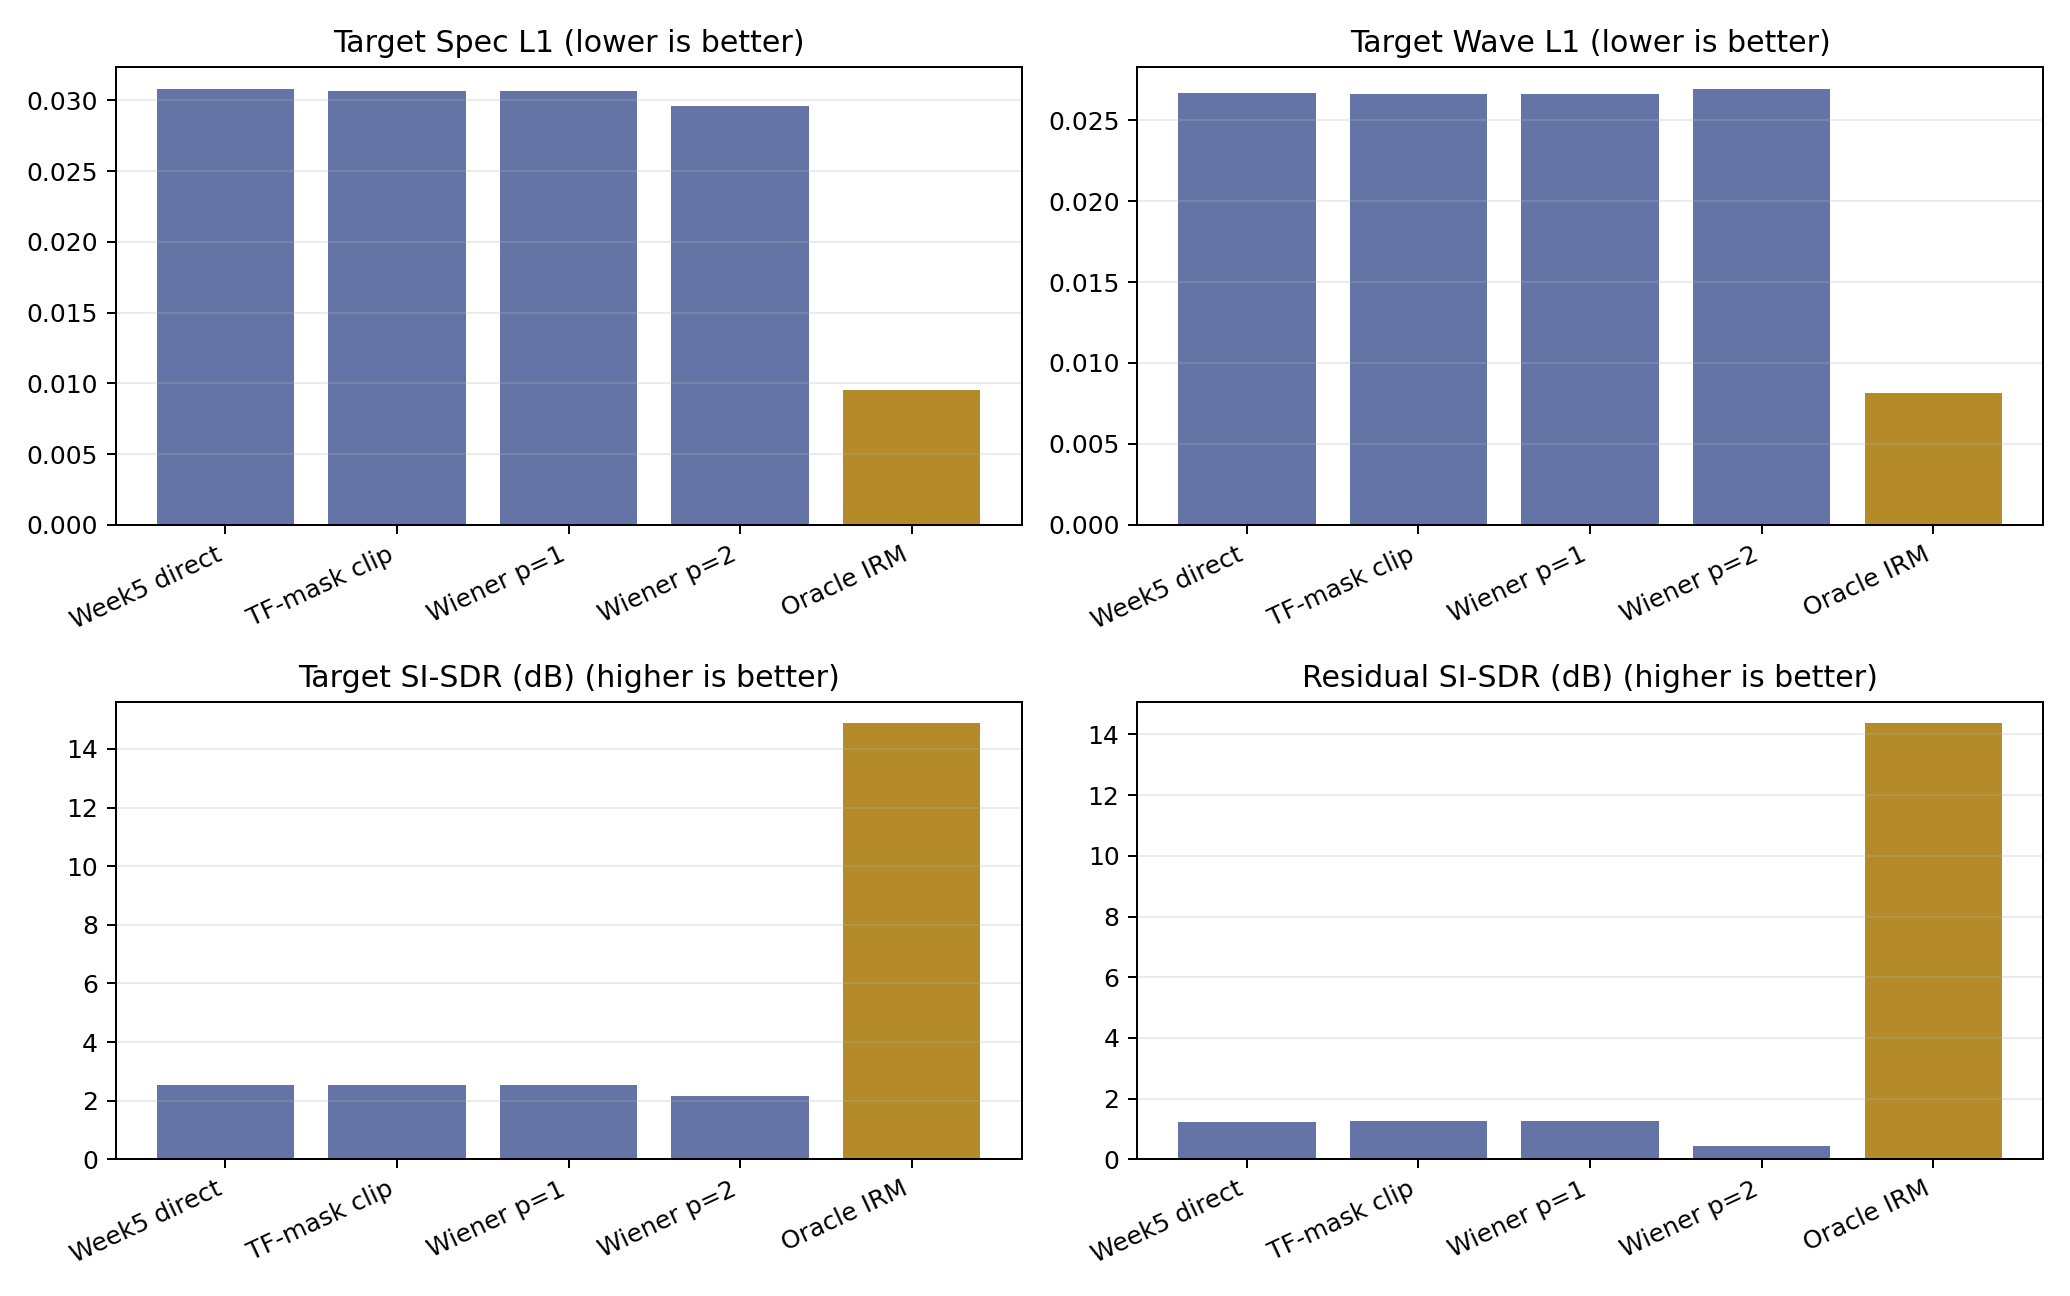
\includegraphics[width=0.88\textwidth]{irm_ft_metrics.png}
  \caption{IRM continued training后的direct、TF-mask、Wiener和Oracle结果。}
  \label{fig:irm-final}
\end{figure}

表\ref{tab:main-result}汇总了完整测试集的主结果。Mamba主干相对self-attention改善三个target指标；waveform L1继续改善波形和SI-SDR；IRM辅助训练将Target SI-SDR提高到2.535~dB。最终Residual SI-SDR为1.273~dB，低于waveform阶段的1.975~dB。

\begin{table}[H]
  \centering
  \caption{完整test split、1-step inference主结果。}
  \label{tab:main-result}
  \small
  \setlength{\tabcolsep}{4pt}
  \resizebox{\textwidth}{!}{\begin{tabular}{lrrrrr}
    \toprule
    Model & Params & Spec L1$\downarrow$ & Wave L1$\downarrow$ & Target SI-SDR$\uparrow$ & Residual SI-SDR$\uparrow$ \\
    \midrule
    Self-attention baseline & 3.103M & 0.03539 & 0.03203 & $-0.419$ & -- \\
    Self-attention recheck & 3.103M & 0.03600 & 0.03378 & $-1.418$ & -- \\
    Mamba-style SSM & 3.015M & 0.03047 & 0.02815 & 0.642 & 1.743 \\
    Mamba + waveform L1 & 3.015M & 0.03097 & 0.02721 & 1.417 & \textbf{1.975} \\
    Mamba + IRM FT + TF-mask & 3.015M & 0.03064 & \textbf{0.02663} & \textbf{2.535} & 1.273 \\
    \bottomrule
  \end{tabular}}
\end{table}

\begin{figure}[H]
  \centering
  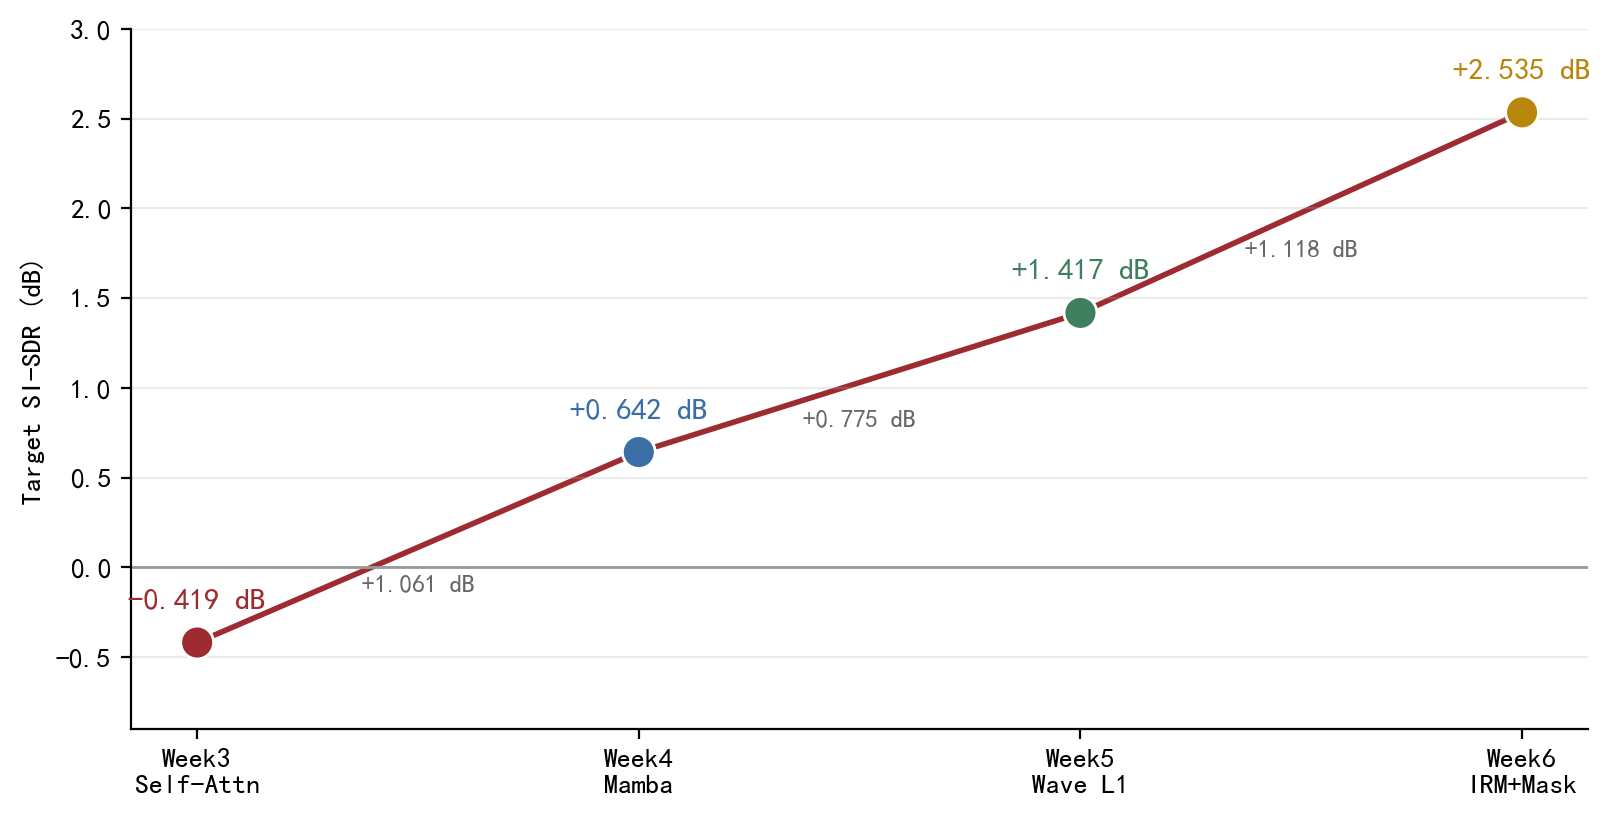
\includegraphics[width=0.84\textwidth]{si_sdr_progression.png}
  \caption{从baseline到最终模型的Target SI-SDR变化。}
  \label{fig:progression}
\end{figure}

Residual指标下降揭示了当前输出结构的局限。训练损失集中约束target幅度、target波形和target mask，residual仅通过相减产生。target输出中与参考方向一致的变化可能提高其SI-SDR，同时改变误差在residual中的投影。mixture consistency仍然接近数值精度，二源各自的感知质量没有得到联合保证。

\subsection{类别差异}

最终模型按target label统计后，vacuum cleaner的平均SI-SDR为8.41~dB，rain为4.33~dB；keyboard typing和clock tick分别为$-1.55$~dB和$-0.28$~dB。图\ref{fig:classwise}展示了全部类别的结果。

\begin{figure}[H]
  \centering
  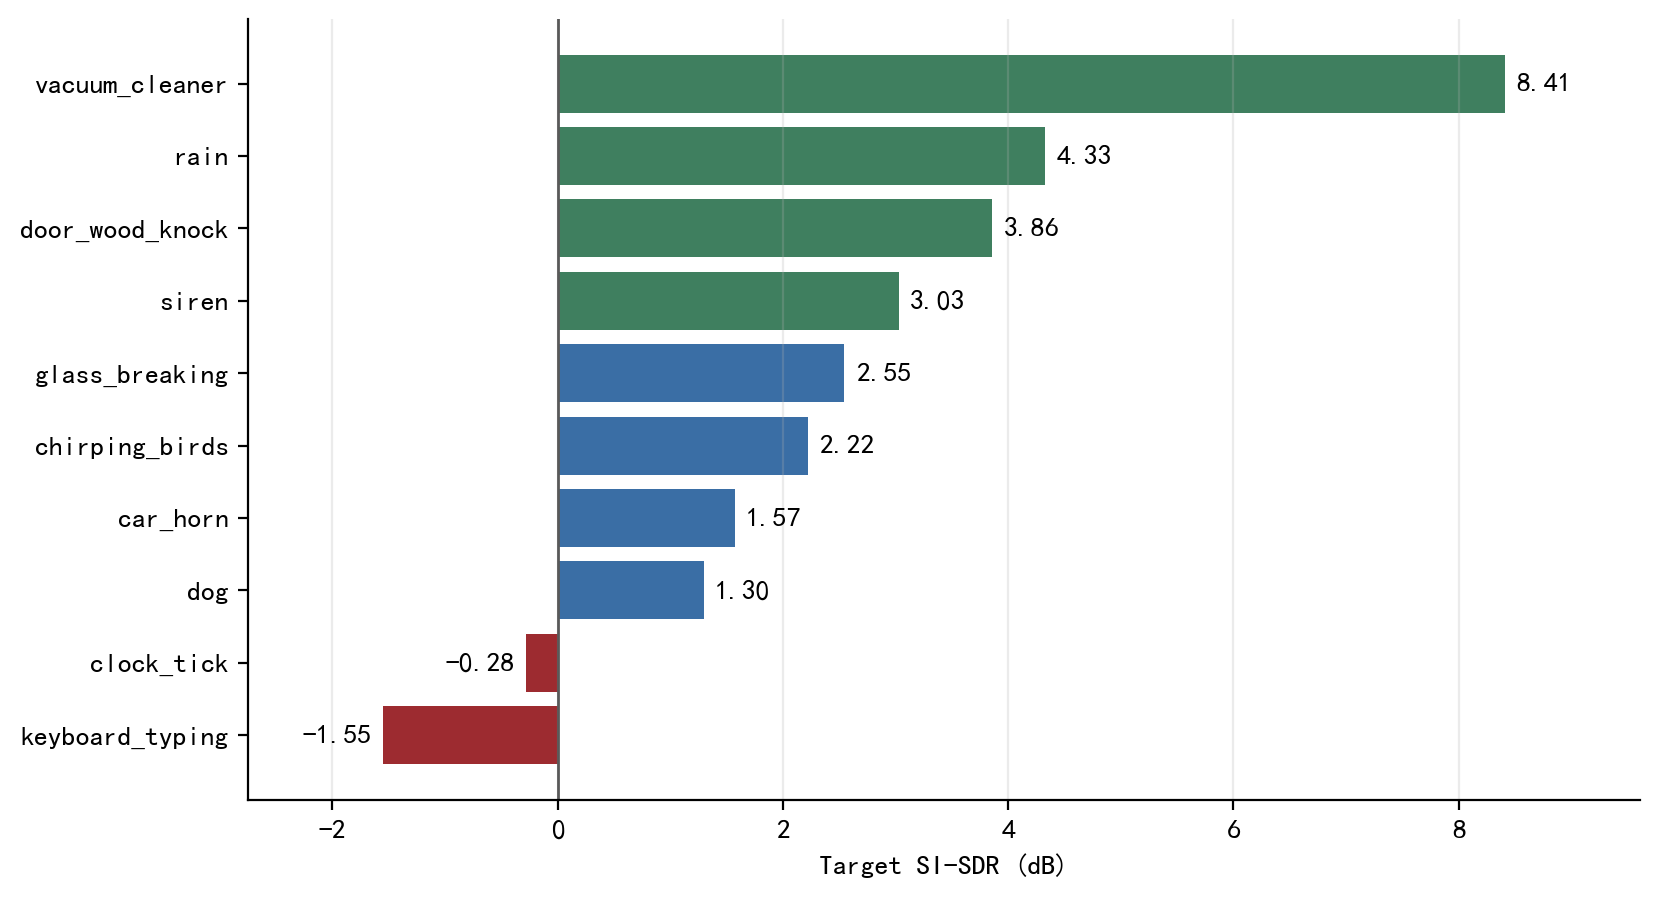
\includegraphics[width=0.88\textwidth]{classwise_week6.png}
  \caption{最终模型按target label统计的Target SI-SDR。}
  \label{fig:classwise}
\end{figure}

一种可能的解释来自时间结构。持续声在多个相邻STFT帧中保持相近纹理，模型能够从更多位置获得一致信息；瞬态声只覆盖少量帧，被另一声源遮挡后更难恢复。car horn与siren的谐波区域也可能发生重叠。当前类别样本数有限，这些分析用于解释现象，仍需更多随机种子和更大数据集验证。

\subsection{成功、失败与边界样例}

随包保留的成功样例均来自test split。vacuum cleaner与clock tick混合时，target SI-SDR为15.52~dB；door wood knock与glass breaking混合时为13.62~dB；rain与dog混合时为11.95~dB。这些记录覆盖了持续声和瞬态声，音频与频谱图位于\code{samples\_demo/}。

失败样例主要落在三种情况。第一类是target能量弱，例如clock tick被更强的vacuum cleaner覆盖，模型倾向于保留连续背景。第二类是两个源频谱重叠，例如siren与car horn都含有较强谐波，label条件无法完全消除局部混淆。第三类是强瞬态，例如glass breaking只在短时间内出现，模型对关键帧的削弱会显著影响听感。

边界样例也值得保留。有些记录的Spec L1变好，SI-SDR却下降；另一些记录呈现相反趋势。这些样例表明平均幅度误差、波形误差和投影信噪比各自关注不同方面。我们在模型筛选时采用多指标并列，最终结论以完整测试集平均值和试听结果共同支撑。

\section{讨论}

\subsection{我们从算子比较中学到了什么}

Mamba-style SSM在当前约3M参数设置下表现优于self-attention，直接证据是Target Spec L1、Wave L1和SI-SDR同时改善。self-attention通过两两注意力建立全局交互，当前selective SSM则沿token顺序递推状态。现有实验只能确认两种实现的结果差异，尚不能区分顺序归纳偏置、优化稳定性和参数分配各自贡献了多少。

实验没有覆盖更深的Transformer、不同patch顺序、相同FLOPs或多个随机种子，因而算子结论仍有边界。课程项目中我们优先控制参数量、batch、数据和推理方式，得到了一组可复现的局部证据。更严格的研究需要增加强U-Net、Conv-TasNet、SepFormer等基线，并报告多次训练的均值和方差。

\subsection{损失函数与评价指标的关系}

baseline阶段的结果显示，目标函数和最终评价之间存在距离。Spec L1把每个时频格子同等对待，平滑预测可能降低平均误差；SI-SDR关注目标投影与剩余误差的能量比例，对局部泄漏、相位失真和幅度偏差更敏感。waveform L1把iSTFT重建纳入训练，最终音频指标随之改善。

IRM辅助损失又增加了一层结构约束。它要求预测幅度相对mixture形成合理比例，训练时利用两个stem提供的监督。TF-mask单独使用几乎没有改变结果，说明waveform模型的大多数预测已经接近有界区域；IRM训练改变了模型对时频格子的分配方式，Target SI-SDR才出现较大提升。

\subsection{相位与表示空间的限制}

当前系统对target phase没有建模。mixture phase包含两个源叠加后的相位关系，某个源占主导的时频格子上近似较好，重叠区域误差会更明显。Oracle IRM达到14.869~dB而未接近无穷，也由此可以理解：理想幅度mask仍要借用mixture phase，iSTFT得到的波形与真实target保留差异。

继续留在频谱域时，可以预测phase-sensitive mask、complex ratio mask或直接回归复数STFT。另一种选择是使用U-Net，它的多尺度卷积和skip connection更贴合频谱图局部结构。若继续使用DiT，可先训练VAE把波形或频谱压缩到低维latent，再在隐空间做Flow Matching。SAM Audio采用的大规模latent DiT路线说明这种组合具有扩展潜力，所需数据和算力远高于本项目。

\begin{figure}[H]
  \centering
  \begin{tikzpicture}[node distance=8mm]
    \node[spec,align=center] (cur) {当前系统\\频谱域幅度 + mixture相位};
    \node[mix,above right=6mm and 14mm of cur,text width=32mm,align=center] (unet) {频谱 U-Net\\多尺度卷积与skip更贴合局部结构};
    \node[mlp,right=16mm of cur,text width=32mm,align=center] (latent) {VAE latent DiT\\先压缩再在隐空间做Flow Matching};
    \node[good,below right=6mm and 14mm of cur,text width=32mm,align=center] (phase) {phase-aware\\复数谱 / PSM，补上相位};
    \draw[flowarr] (cur) -- (unet);
    \draw[flowarr] (cur) -- (latent);
    \draw[flowarr] (cur) -- (phase);
  \end{tikzpicture}
  \caption{沿频谱U-Net、latent DiT和phase-aware建模继续推进的三条路径。}
  \label{fig:future}
\end{figure}

\subsection{有效性与局限}

实验采用固定manifest、官方fold和统一的full test split，主结果使用同一1-step协议。各阶段只改变一个主要因素：序列mixer、waveform辅助损失或IRM辅助损失。Oracle结果单独列为诊断参考，未计入模型成绩；residual下降也在主表中保留。

不足同样明确。数据来自10类合成2-mix，真实环境中的混响、背景噪声、未知类别和多于两个声源尚未覆盖。每个主模型只训练一次，随机波动没有通过多seed实验估计。self-attention与Mamba参数量接近，计算量和训练时长未做到严格等值。Mamba-style实现使用显式PyTorch状态递推，功能上体现选择性SSM，运行效率无法代表官方融合kernel。最终输出仍是单target头，residual subtraction缺少独立监督。

\subsection{后续工作}

若继续推进，我们会先建立一个强频谱U-Net对照，并在同一ESC-50 2-mix协议下比较参数量、SI-SDRi和推理速度。第二步尝试复数频谱或phase-sensitive目标，观察mixture phase造成的误差能否被削弱。第三步把target与residual改成联合输出，在loss中同时约束两路SI-SDR和mixture consistency。数据侧可扩展到FUSS等通用声音分离benchmark，报告标准化SI-SDRi，并加入真实录音和更多源数。

若保留DiT主线，VAE隐空间值得优先验证。一个可操作的方案是先训练小型音频VAE，测量重建SI-SDR与压缩率，再把当前Conditional Flow Matching迁移到latent token。这样可以把“VAE重建上限”和“DiT分离能力”拆开评价，也能判断当前瓶颈究竟来自高维频谱、模型容量还是数据规模。

\subsection{复现说明}

留档代码按照实验阶段保留数据构造、baseline、Mamba、waveform continued training和IRM continued training。原始ESC-50和生成后的2-mix音频没有放进邮件材料，数据来源、许可和下载地址记录在提交目录的\code{数据来源.txt}。下载ESC-50后，在\code{代码与模型}目录执行数据管线即可重新产生clean source、mixture和manifest。

\begin{table}[H]
  \centering
  \caption{主要复现材料。}
  \label{tab:reproduce}
  \small
  \begin{tabularx}{0.95\textwidth}{p{4.0cm}X}
    \toprule
    内容 & 相对路径 \\
    \midrule
    数据构造配置 & \code{week2/configs/esc50\_2mix.yaml} \\
    Self-attention配置 & \code{week3/configs/minidit\_self\_attention.yaml} \\
    Mamba配置 & \code{week4/configs/minidit\_mamba.yaml} \\
    Waveform训练配置 & \code{week5/configs/mamba\_waveform\_finetune.yaml} \\
    IRM训练与TF-mask评估 & \code{week6/scripts/} \\
    最终模型权重 & \code{checkpoint/week6\_best.pt} \\
    已保存测试结果 & \code{results/} \\
    \bottomrule
  \end{tabularx}
\end{table}

Week6评估脚本通过\code{--checkpoint}参数加载最终权重。完整测试包含2,000条test target records，本地CPU运行时间较长。留档包已经保存各阶段的summary JSON、按类别CSV、推理步数消融和训练metrics，报告中的表格均可追溯到这些文件。

LaTeX源稿、参考文献和图件位于\code{report\_source/}。在该目录运行\code{latexmk -xelatex main.tex}即可重新编译报告。代码依赖列在\code{requirements.txt}中，核心运行环境为Python、PyTorch、NumPy、SciPy、SoundFile、PyYAML和tqdm。

\section{结论}

本文完成了一个类别条件的环境声音二源分离系统。ESC-50中的10类clean source被合成为训练、验证和测试2-mix；模型在log-magnitude STFT上学习从mixture到target的Conditional Flow Matching路径；预测幅度与mixture phase组合后恢复波形，residual由mixture减去prediction target得到。

实验从self-attention Mini-DiT baseline出发。baseline的Target SI-SDR为$-0.419$~dB，Mamba-style SSM在相近参数量下提高到0.642~dB，加入waveform L1 continued training后达到1.417~dB。TF-mask单独后处理带来的变化很小，Oracle IRM显示mask监督仍有空间。最终IRM辅助训练加TF-mask取得2.535~dB Target SI-SDR和0.02663 Wave L1。

在当前轻量设置下，选择性状态空间mixer、音频域辅助损失和IRM监督均改善了target分离。Residual SI-SDR下降、瞬态类别表现偏低以及mixture phase带来的重建误差表明，单target幅度预测仍有明显限制。后续研究可比较频谱U-Net、联合双输出、复数频谱和VAE latent DiT。

\clearpage
\appendix
\section{关键配置汇总}

为了便于核对实验口径，表\ref{tab:appendix-feature}和表\ref{tab:appendix-model}集中列出特征、模型与评估配置。各阶段YAML文件保留了完整参数，以下数值覆盖报告中的全部主结果。

\begin{table}[H]
  \centering
  \caption{音频与频谱配置。}
  \label{tab:appendix-feature}
  \begin{tabular}{ll}
    \toprule
    项目 & 设置 \\
    \midrule
    Sample rate & 16,000 Hz \\
    Duration & 5 s / 80,000 samples \\
    Channels & Mono \\
    STFT & $n_{\mathrm{fft}}=1024$, hop $=256$, win $=1024$ \\
    Spectrogram size & $513\times313$ \\
    Representation & Scaled $\log(1+|\mathrm{STFT}|)$ \\
    Reconstruction phase & Mixture phase \\
    Flow start & Mixture spectrogram \\
    Inference & 1-step Euler \\
    \bottomrule
  \end{tabular}
\end{table}

\begin{table}[H]
  \centering
  \caption{Mini-DiT与训练配置。}
  \label{tab:appendix-model}
  \begin{tabular}{ll}
    \toprule
    项目 & 设置 \\
    \midrule
    Hidden size / depth & 192 / 4 \\
    Patch size & $16\times16$ \\
    Attention heads & 6 \\
    MLP ratio & 4.0 \\
    Mamba state / convolution & 16 / 4 \\
    Trainable parameters & 3,014,977 (Mamba), 3,102,529 (self-attention) \\
    Optimizer & AdamW, weight decay 0.01 \\
    Gradient clipping & 1.0 \\
    Waveform loss weight & 0.1 \\
    IRM loss weight & 0.1 \\
    Full test records & 2,000 \\
    \bottomrule
  \end{tabular}
\end{table}

留档权重对应IRM continued training第2个epoch。该权重加载后共有3,014,977个可训练参数，评估脚本会根据label逐条生成target，并通过mixture subtraction得到residual。主结果、mask消融和类别统计均已在\code{results/}中保存。

\clearpage
\bibliographystyle{unsrt}
{\footnotesize\bibliography{references}}

\end{document}
